%%%%%%%%%%%%%%%%%%%%%%%%%%%%%%
%
%		Master thesis report
% 	Visualisation of Gene Ontology and Cluster Analysis Results
%	Author: Vladyslav Aleksakhin

\documentclass[12pt]{article}

\usepackage{geometry}
\usepackage{tabularx}
\usepackage{graphicx}
\usepackage{subfig}
\usepackage{url}
\usepackage{color}
\usepackage{listings}

\geometry{
  oneside,
  a4paper,
  left=3cm,
  right=3cm,
  top=2cm,
  bottom=2.5cm,
  hcentering,
  nohead
}

\makeatletter
\renewcommand{\subsection}{
    \@startsection
    {subsection}
    {2}
    {\z@}
    {-3.5ex \@plus -1ex \@minus -.2ex}
    {2.3ex \@plus.2ex}
    {\normalfont\normalsize\bfseries}
}
\makeatother

\makeatletter
\renewcommand{\subsubsection}{
    \@startsection
    {subsubsection}
    {3}
    {\z@}
    {-3.5ex \@plus -1ex \@minus -.2ex}
    {2.3ex \@plus.2ex}
    {\normalfont\normalsize\bfseries}
}
\makeatother


\newcommand*{\mywebref}[3]{
	\bibitem{#1} #2 is available on the web \url{#3}. Last access in December 2011.
}

\newcommand*{\todo}[1]{
	\begin{LARGE}
		\textcolor{red}{#1}
	\end{LARGE}
}

\newcommand*{\mysection}[2]{
  \newpage
  \section{#1}
  \label{#2}
  \setcounter{figure}{0}
}

\newcommand*{\myappendix}[1]{	
	\addtocounter{section}{1}

	\section*{Appendix \Alph{section}: #1}	
	\addcontentsline{toc}{section}{Appendix \Alph{section}: #1}

	\renewcommand{\thesection}{\Alph{section}}
	\renewcommand{\thefigure}{\thesection.\arabic{figure}}

	\setcounter{figure}{0}
}

\renewcommand{\thefigure}{\thesection.\arabic{figure}}

\begin{document}

\pagenumbering{roman}

\begin{titlepage}
\begin{center}

\Huge{Visualization of Gene Ontology and Cluster Analysis Results}

\vfill

\begin{Large}
Master's Thesis Report (30 credit points)

\vfill

Supervisor: Prof. Dr. Andreas Kerren\\
Co-Supervisor: Ilir Jusufi\\
Student: Vladyslav Aleksakhin

\vfill

Linnaeus University\\
School of Computer Science, Physics and Mathematics

\end{Large}


\end{center}
\end{titlepage}


\newpage
\section*{Abstract}

The task of the thesis is a new visualization method. Gene Ontologies and hierarchical clustering are both important tools in biology and medicine to study high-throughput data such as transcriptomics and metabolomics data. Enrichment of ontology terms in the data is used to identify statistically overrepresented ontology terms, giving insight into relevant biological processes or functional modules. Hierarchical clustering is a standard method to analyze and visualize data to find relatively homogeneous clusters of experimental data points. Both methods support the analysis of the same data set, but are usually considered independently. However, often a combined view is desired: visualizing a large data set in the context of an ontology under consideration of a clustering of the data.

\newpage
\section*{Acknowledgments}
\label{sec:acknowledgments}

I would like to express my gratitude to my supervisor Dr. Andreas Kerren and to my co-supervisor Ilir Jusufi. They encouraged and stimulated me in each step of this work. Moreover, my greatest gratitude goes to my family that made my study possible, for their constant moral support even though thousands of kilometers separated us. Finally, I would like to thank to my best friend Olga for support and patience.

\newpage
\tableofcontents

\setcounter{page}{1}
\pagenumbering{arabic}

\section{Introduction}
\label{sec:introduction}

\subsection{Motivation}
\label{sec:motivation}

Computer information analysis is the only known approach to work with huge amount of data produced every day. In any field of human work there is data and there are tasks of analyzing it. The topic of this thesis combines two areas of data computing: information visualization and biological data processing.

There are many datasets for analysis in biology. This thesis is intended to make a visualization tool for genes and gene relations in order to help biologists with their work. Data for processing was provided by the Plant Bioinformatics Group of Leibniz Institute of Plant Genetics and Crop Plant Research (IPK), Germany. Data consists of Gene Ontologies and hierarchical clustering which are are both important tools in biology and medicine for high-throughput data study.

To help analyzing this data the following approaches are desired: visualizing the data set in the context of a ontology (such as the Gene Ontology) and in the context of data clustering. There is no solutions that deals with combined visualization of ontology (DAG) and an hierarchical clustering (tree) of one data set. The aim of this work is creation of a new visualization approach and is implementation in order to provide a useful tool for biologists in their everyday research work.

The result of this work is a base of the research paper --- \textsf{Ilir Jusufi, Andreas Kerren, Vladyslav Aleksakhin, and Falk Schreiber. Visualization of Mappings between the Gene Ontology and Cluster Trees. Conference on Visualization and Data Analysis 2012 (EI-107) Part of IS&T/SPIE Electronic Imaging 2012 (Jan 22-26, 2012) VDA 2012 Dates: January 23-25, 2012.}

\subsection{Thesis Collaboration}
This project is the result of collaboration between ISOVIS research group (Head: Prof. Dr. Andreas Kerren~\cite{Kerren}) of Linn\ae us University at V\"axj\"o, Sweden, and Plant Bioinformatics Group (Head: Prof. Dr. Falk Schreiber~\cite{Schreiber}) of Leibniz Institute of Plant Genetics and Crop Plant Research (IPK), Germany.


ISOVIS research group is focused on the exploration analysis and visualization of large information data in Software Engineering, Geography, or Biology. There are several different techniques for information visualization, one of them is widely used in the research is Human-Centered Visualization. This kind of visualization combines different research areas: Information Visualization, Scientific Visualization, Human-Computer Interaction, Data Mining, Information Design, Graph Drawing, and Computer Graphics.


As said on official page of Plant Bioinformatic Group:
\begin{quotation}
``The research group focuses on modeling, analysis, simulation and visualization of biological networks in the context of plant biological problems.
Our aim is the development of methods and software tools for the analysis of complex biological networks.
Therefore we integrate, process and analyze data from different areas of genome, proteome and metabolome research and present the results in a user-friendly way.
The emphasis is on the linkage of experimental data about expression profiles and metabolite patterns with metabolic and regulatory networks.
The data and complex connections are modeled using graphs. We are developing graph (network) analysis and interactive visualization methods to discover network properties and to make the data easily accessible to the user.
A subsequent step is to use the data for the simulation of metabolic and regulatory networks.''~\cite{PBG}
\end{quotation}


\subsection{Thesis Outline}
\label{sec:structure}

Section~\ref{sec:introduction} explains the problem, thesis purpose and collaboration. Section~\ref{sec:background} presents the results of the related work, where relevant research efforts in the fields of Bioinformatic, Information Visualization and Bio Visualization were explored in connection to the thesis work. Section~\ref{sec:algorithm} covers the following topics: visualization complexity and describes the goals, description of the input data and mapping between graphs. Section~\ref{sec:solution} describes attempt to the visualization solution, the solution for Cluster Ananlysis tree and the visualization solution for Gene Ontology visualization technique. One of the biggest section in the report is Section~\ref{sec:implementation} that determines the requirements, use cases, and proposes the architecture for thesis application.
Additionally in Section~\ref{sec:solution} describes the input data format overview, overview of the different graph file formats, implementation details, architecture of the system, used libraries, project management tools. Technical details of the visualization algorithms are explained in Sections~\ref{sec:cluster} and~\ref{sec:go}. Last part of the report is Section~\ref{sec:conclusion} that describes problems and future work.

\newpage
\section{Background}
\label{sec:background}


\subsection{Information Visualization}
\label{sec:infovis}

The field of computer-based information visualization draws on ideas from several intellectual traditions: computer science, psychology, semiotics, graphic design, cartography, and art.
The two main threads of computer science relevant for visualization are computer graphics and human-computer interaction.
The areas of cognitive and perceptual psychology offer important scientific guidance on how humans perceive visual information.
A related conceptual framework from the humanities is semiotics, the study of symbols and how they are convey meaning.
Design, as the name suggests, is about the process of creating artifacts well- suited for their intended purpose.
Cartographers have a long history of creating visual representations that are carefully chosen abstractions of the real world.
Finally, artists have refined methods for conveying visual meaning in sub-disciplines ranging from painting to cinematography.

Information visualization has gradually emerged over the past fifteen years as a distinct field with its own research agenda.
The distillation of results from areas with other goals into specific prescriptive advice helping us to design and evaluate visualization systems is nontrivial.
Although these traditions have much to offer, effective synthesis of such knowledge into a useful methodology.

The standard argument for visualization is that exploiting visual processing can help people explore or explain data. We have an active field of study because the design challenges are significant and not fully understood. Questions about visual encoding are even more central to information visualization than to scientific visualization.
The subfield names grew out of an accident of history, and have some slightly unfortunate connotations when juxtaposed:
information visualization is not unscientific, and scientific visualization is not uninformative.
The distinction between these two is still not agreed on by all, but the definition used here is that information visualization hinges on finding a spatial mapping of data that is not inherently spatial,
whereas scientific visualization uses a spatial layout that is implicit in the data.

\begin{figure}[h!]
\centering
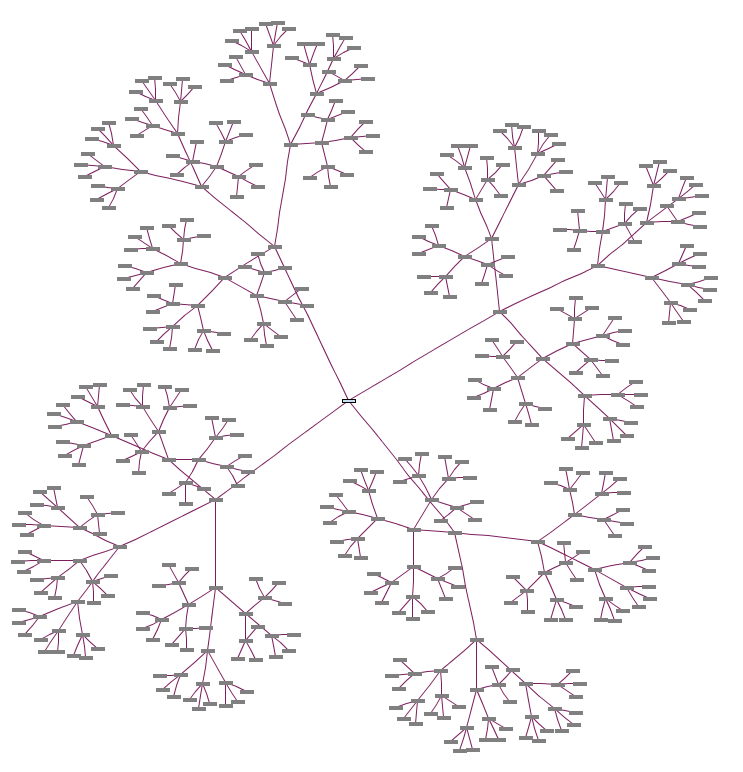
\includegraphics[scale=0.3]{pictures/Tree_graph_example.png}
\caption{Sample visualisation of the tree graph}
\label{fig:tree_graph_example}
\end{figure}

\begin{quotation}
``Graph drawing or Graph layout, as a branch of graph theory, applies topology and geometry to derive two-dimensional representations of graphs.
A drawing of a graph is basically a pictorial representation of an embedding of the graph in the plane (generally, with edge intersections allowed),
usually aimed at a convenient visualization of certain properties of the graph in question or of the object modeled by the graph.
Graph drawing is motivated by applications such as Very-large-scale (VLSI)~\cite{VLSI} integration circuit design, social network analysis,
cartography, and bioinformatics, many of which make use of information visualization.''~\cite{Graph_drawing}
\end{quotation}

There are many methods and approaches to graph visualization. They are all based on various perception qualities of human.
The Radial Dendrograms~\cite{Radial_dendrogram} algorithm is used for results of cluster analysis visualization.

Dendrogram~\cite{Dendrogram} plot is one of the visualization algorithm for hierarchical structures. It illustrating the outcome of decision tree-type clustering in statistics.
Most commonly, dendrograms are drawn in a Cartesian layout, as an upright tree. However, this layout does not make good use of space, it is sparse towards the root and crowded towards the leaf nodes.
The spacing between nodes at different levels in the hierarchy is not uniform, which is due to the shrinking number of nodes from bottom to top. For this reason, long, wide-spanning connecting lines are needed to merge nodes at higher levels.
A better layout in this respect is a polar or a radial layout, where leaf nodes are located on the outer ring and a root is located in the center, as a focal point.
A more uniform node spacing results are leading to a better utilization of space and resulting to a better illustration of the class relationships.
Recently, Barlow and Neville~\cite{Barlow_Neville} presented an empirical user study for tree layouts (with less than 200 leaves) in which they compare some of the major schemes: the organizational chart (a standard drawing of a tree),
the tree ring (basically a pie chart of circular segments), the icicle plot (the cartesian version of the tree ring), and the tree map. According to the measured performance within a group of 15 users,
the three former methods yielded similar results where the icicle plot has a slight advantage. However, given larger number of leaves in our case (1000 and more) and the fact that the tree ring is the most compact of the three winning configurations,
a radial layout seemed to be the most favorable one for our purpose. Radial graph layouts that illustrate hierarchical relationships are very popular, and for the special application of dendrograms.
We know only one other application that uses a radial layout. The recent one by Kreussler and Schumann~\cite{Kreussler_Schumann} that mentioned before, users often would like to focus on certain portions of the display,
while compressing others, without losing context. Fisheye lenses and hyperbolic zooming were proposed to provide these capabilities.
In the context of tree rings Yang, Ward and Rundensteiner~\cite{Yang_Ward} proposed a system in which users may either perform a polar zoom (i.e. expand the width of one or more adjacent rings while reducing others) or
a radial zoom (i.e. expand the arc angle of some adjacent segments while reducing others). More over, users can perform these operations by pinning down one ring or arc segment and dragging another.
A limiting factor here is that users cannot perform both operations simultaneously that can be awkward in certain instances. To address this shortcoming
our application generalizes these concepts by allowing arbitrary warps of the dendrogram domain, i.e. we allow radial and polar zooms simultaneously.


\subsection{Bioinformatics}
\label{sec:bioinformatics}

In the last few decades, advances in molecular biology and the equipment available for research in this field have allowed the increasingly rapid sequencing of large portions of the genomes of several species.
In fact, to date, several bacterial genomes, as well as those of some simple eukaryotes (e.g., Saccharomyces cerevisiae, or baker's yeast) have been sequenced in full.
The Human Genome Project, designed to sequence all 24 of the human chromosomes, is also progressing. Popular sequence databases, such as GenBank and EMBL, have been growing at exponential rates.
This deluge of information has necessitated the careful storage, organization and indexing of sequence information. Information science has been applied to biology to produce the field called Bioinformatics.


The simplest tasks used in bioinformatics concern the creation and maintenance of databases of biological information.
Nucleic acid sequences (and the protein sequences derived from them) comprise the majority of such databases. While the storage and or organization of millions of nucleotides is far from trivial,
designing a database and developing an interface whereby researchers can both access existing information and submit new entries is only the beginning.
The most pressing tasks in bioinformatics involve the analysis of sequence information.~\cite{Biology}
Here we can find short introduction and history of Bioinformatics:

\begin{quotation}
``Bioinformatics is the application of information technology to the field of molecular biology.
The term bioinformatics was coined by Paulien Hogeweg in 1978 for the study of informatic processes in biotic systems.
Bioinformatics now entails the creation and advancement of databases, algorithms, computational and statistical techniques, and theory to solve formal and practical problems arising from the management and analysis of biological data.
Over the past few decades rapid developments in genomic and other molecular research technologies and developments in information technologies have combined to produce a tremendous amount of information related to molecular biology.
It is the name given to these mathematical and computing approaches used to glean understanding of biological processes.
Common activities in bioinformatics include mapping and analyzing DNA and protein sequences, aligning different DNA and protein sequences to compare them and creating and viewing 3D models of protein structures.''~\cite{Bioinformatic}
\end{quotation}

More resources about Bioinformatic are available here~\cite{Bioinformatic_resources}.
The primary goal of bioinformatics is to increase our understanding of biological processes.
However, its focus on developing and applying computationally intensive techniques (e.g., data mining, machine learning algorithms, and visualization) to achieve this goal sets it apart from other approaches.
Major research efforts in the field include sequence alignment, gene finding, genome assembly, protein structure alignment, protein structure prediction, prediction of gene expression and protein-protein interactions, genome-wide association studies and the modeling of evolution.

\subsection{Gene Ontology}
\label{sec:gene_ontology}

As stated above, there are different knowledge databases for biologic information storage.
Gene Ontology~\cite{GO_website} project is one of the first-rate international projects.
The Gene Ontology, or GO, is a major bioinformatics initiative to unify the representation of gene and gene product attributes across all species.
The aims of the Gene Ontology project are threefold. Firstly, to maintain and further develop its controlled vocabulary of gene and gene product attributes,
secondly, to annotate genes and gene products, and assimilate and disseminate annotation data,
and thirdly, to provide tools to facilitate access to all aspects of the data provided by the Gene Ontology project.
The GO is part of a larger classification effort, the Open Biomedical Ontologies (OBO)~\cite{OBO}.
The Gene Ontology project provides an ontology of defined terms representing gene product properties.
The ontology covers three domains. First is cellular component and the parts of a cell or its extracellular environment.
Second is molecular function and the elemental activities of a gene product at the molecular level, such as binding or catalysis and biological process.
Finally the third are operations or sets of molecular events with a defined beginning and end, pertinent to the functioning of integrated living units: cells, tissues, organs, and organisms. Each GO term within the ontology has a term name, which may be a word or string of words;
a unique alphanumeric identifier; a definition with cited sources; and a name space indicating the domain to which it belongs.
Terms may also have synonyms, which are classed as being exactly equivalent to the term name, broader, narrower, or related; references to equivalent concepts in other databases;
and comments on term meaning or usage. The GO ontology is structured as a directed acyclic graph, where each term has defined relationships to one or more other terms in the same domain, and sometimes to other domains. The GO vocabulary is designed to be species-neutral,
and includes terms applicable to prokaryotes and eukaryotes, single and multicellular organisms.
The GO ontology is not static, therefore additions, corrections and alterations are suggested by and solicited from members of the research and annotation communities, as well as by those directly involved in the GO project.
For example, an annotator may request a specific term to represent a metabolic pathway, or a section of the ontology may be revised with the help of community experts.
Suggested edits are reviewed by the ontology editors and implemented where appropriate.


\subsection{Clustering}
\label{sec:clustering}

\begin{quotation}
``Data clustering (or just clustering), also called cluster analysis, segmentation analysis, taxonomy analysis, or unsupervised classification,
is a method of creating groups of objects, or clusters, in such a way that objects in one cluster are very similar and objects in different clusters are quite distinct.
Data clustering is often confused with classification, in which objects are assigned to predefined classes. In data clustering, the classes are also to be defined.''~\cite{data_clustering_book}
\end{quotation}

Clustering algorithms can be applied in many fields. For instance:

\begin{itemize}
\item Marketing: finding groups of customers with similar behavior given a large database of customer data that contains their properties and past buying records;
\item Biology: classification of plants and animals given their features;
\item Libraries: book ordering;
\item Insurance: identifying groups of motor insurance policy holders with a high average claim cost, identifying frauds;
\item City-planning: identifying groups of houses according to their house type, value and geographical location;
\item Earthquake studies: clustering observed earthquake epicenters in order to identify dangerous zones;
\item WWW: document classification clustering web log data to discover groups of similar access patterns.
\end{itemize}

\section{Data Extraction}
\label{sec:algorithm}
First step that program supposed to do is to load data and to compute connected components. Data is stored in GML file format. More detail information about this format and other common graph file formats is given in Section~\ref{sec:algorithm}.

\subsection{Dataset Description}
\label{sec:dataset_description}
Gene Ontology data and cluster analysis results presented as directed graphs. They are stored in separate files in special format -- GML files.


GO graph is directed acyclic graph that has 10,042 vertices and  24,155 edges. Also it has 1 root, 2,729 nodes and 7,312 leafs (terminal nodes).
Figure~\ref{fig:yed_GO_vis} shows visualization of the Gene Ontology graph using Hierarchical layout by yEd~\cite{yed} graph editing tool. It obviously shows imperfectness of classic visualization of graphs.


\begin{figure}[h!]
\centering

\includegraphics[scale=0.3]{pictures/yEd_GO.png}
\caption{Gene Ontology yEd visualization}
\label{fig:yed_GO_vis}
\end{figure}


Cluster tree is a directed binary graph that has 14,623 nodes and 14,622 edges. The Cluster graph as a tree has a single root, 7,310 nodes and 7,312 leafs.
To get an impression of the graph, Figure~\ref{fig:Cytoscape_Cluster_1} shows the cluster tree that uses the Cytoscape~\cite{Cytoscape} visualization tool.

\begin{figure}[h!]
\centering
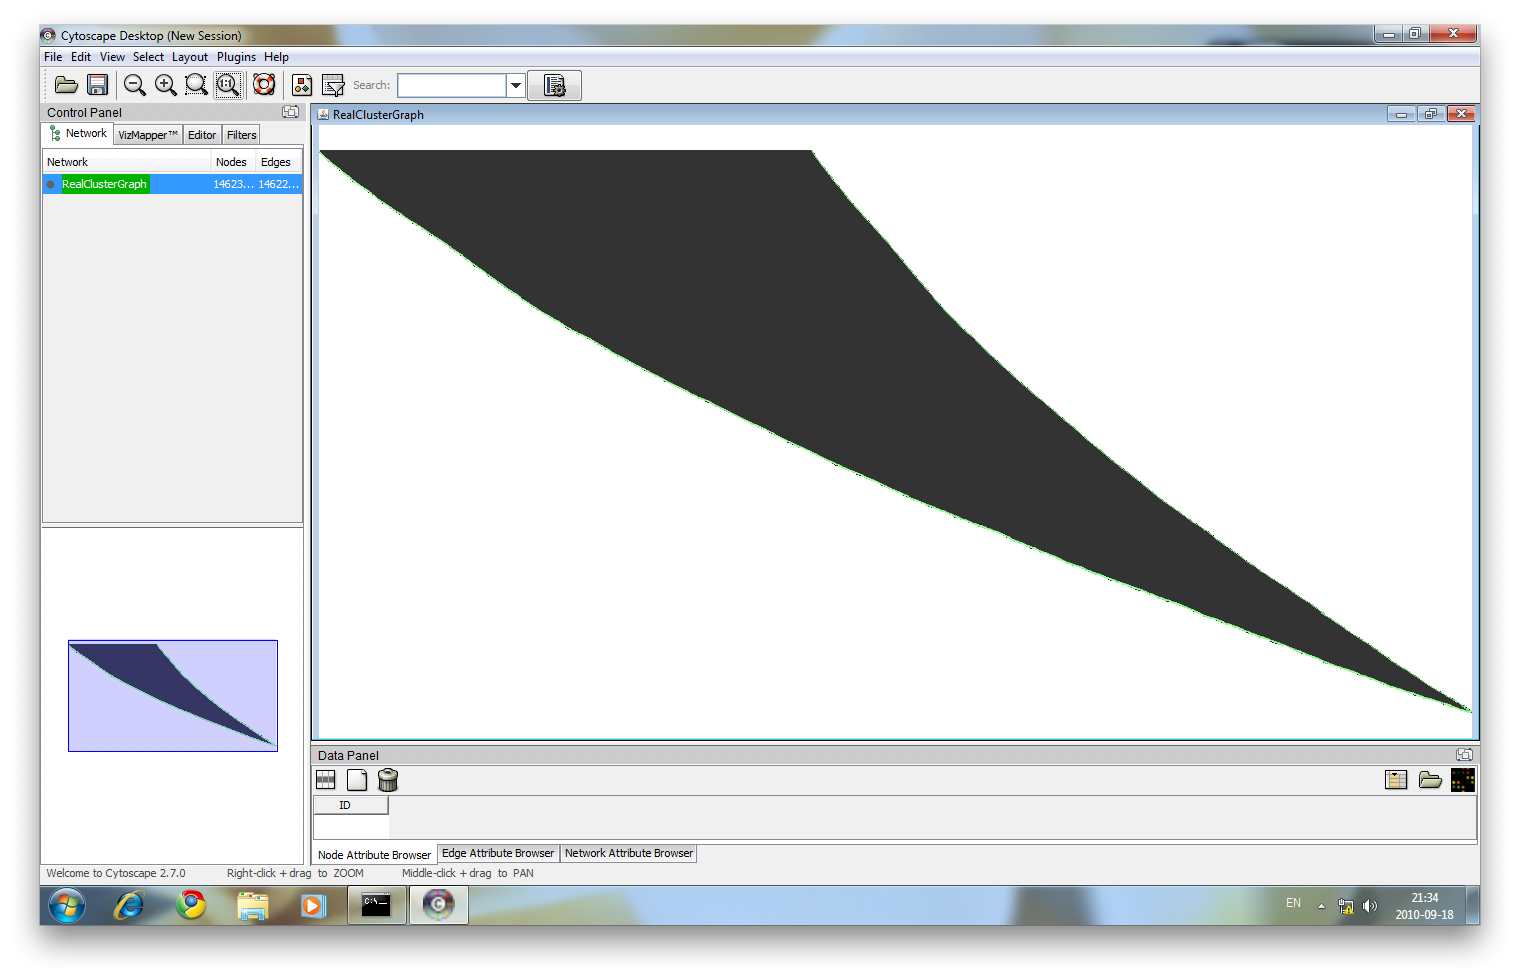
\includegraphics[scale=0.25]{pictures/Cytoscape_cluster_graph_1.png}
\caption{Cluster analysis result tree Cytoscape visualization tool}
\label{fig:Cytoscape_Cluster_1}
\end{figure}

\begin{figure}[h!]
\centering
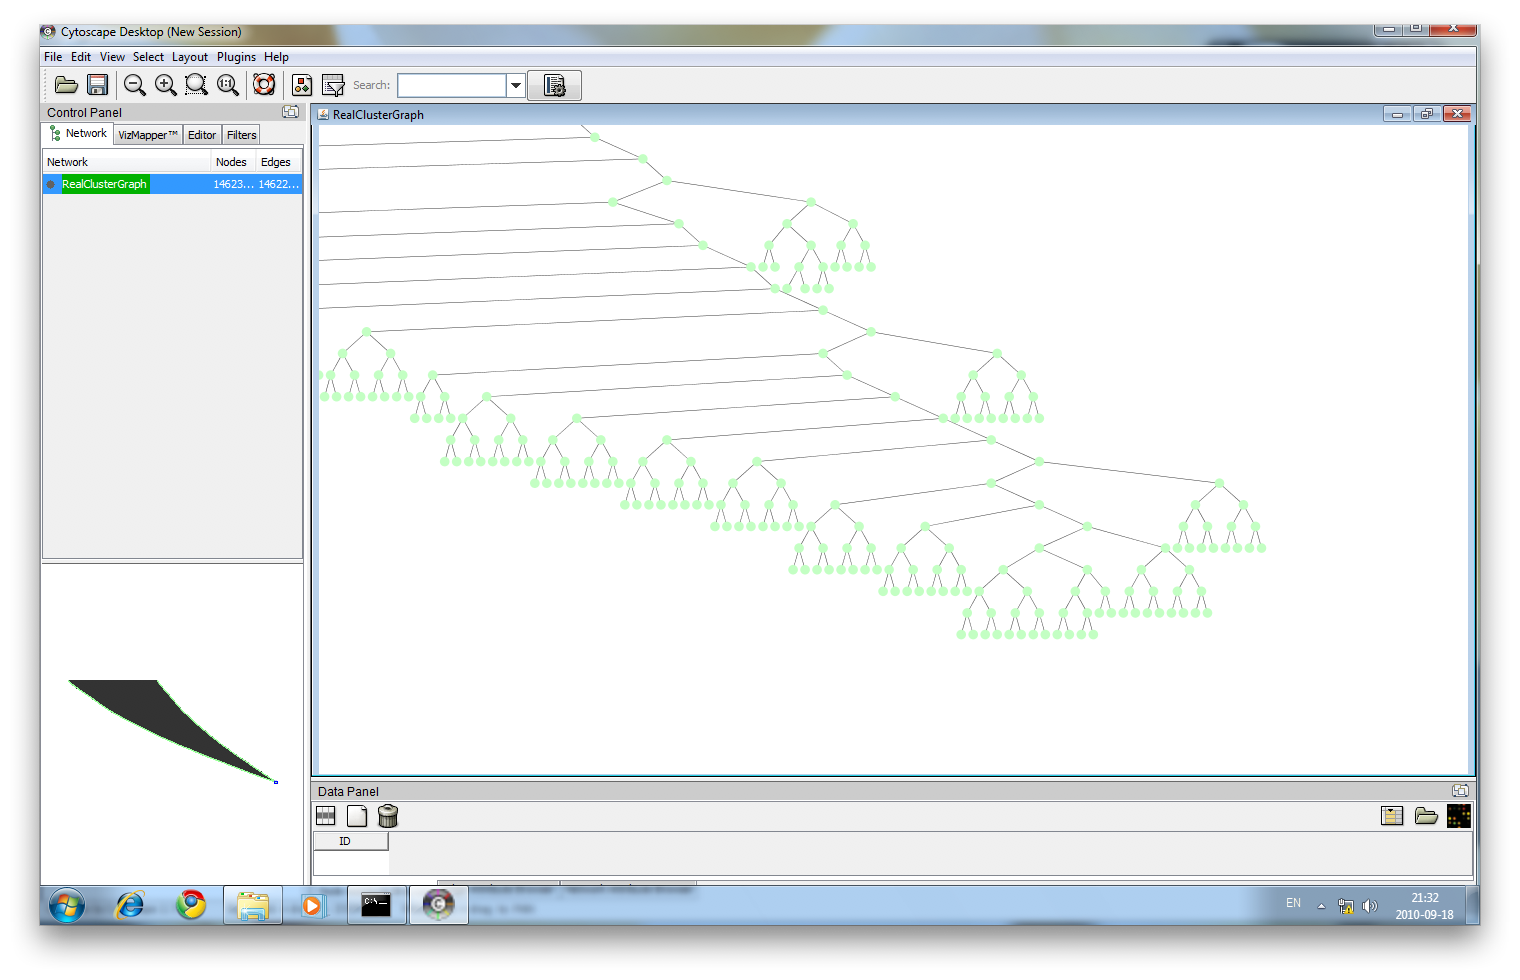
\includegraphics[scale=0.25]{pictures/Cytoscape_cluster_graph_2.png}
\caption{Zoomed cluster analysis result tree}
\label{fig:Cytoscape_Cluster_2}
\end{figure}

Both graphs are independent from each other based on developer point of view: they have different node ids and edge ids. More over, they are connected by vertex labels --
both graphs have same labels for terminal (leaf) vertices. This property is used in the sub-graph extracting algorithm.


Performance is one of the main requirements since the application should work with large quantity of data that has over tens of thousands vertices. It is very important to give a consideration on optimization.


\subsection{Mapping Algorithm}
\label{sec:mapping_algorithm}
Here is the explanation of that program algorithm uses sample graphs:
\begin{enumerate}

\item The program visualizes Gene Ontology and cluster analysis result tree. This visualization technique is discussed in Section~\ref{sec:solution}.

\begin{figure}[h!]
\centering
\subfloat[Selected node in the Gene Ontology]{
    \label{fig:step_1}
    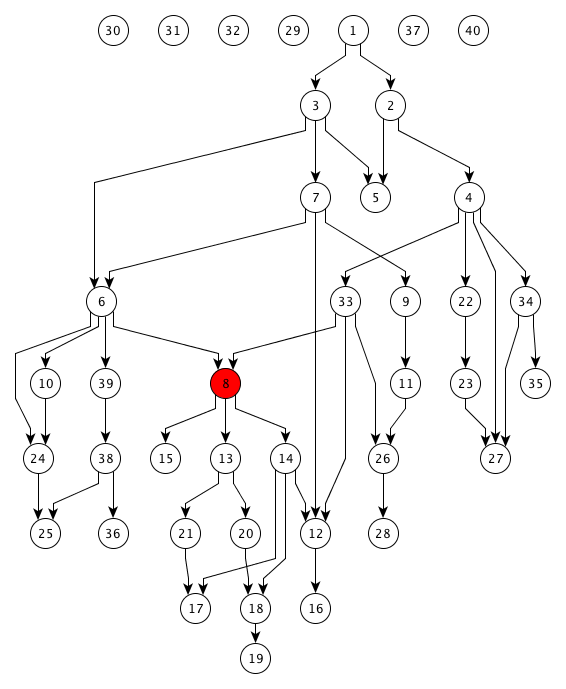
\includegraphics[scale=0.3]{pictures/subgraph_extraction_algorithm_step_1.png}
}
\subfloat[Extract sub-graph for selected node]{
    \label{fig:step_2}
    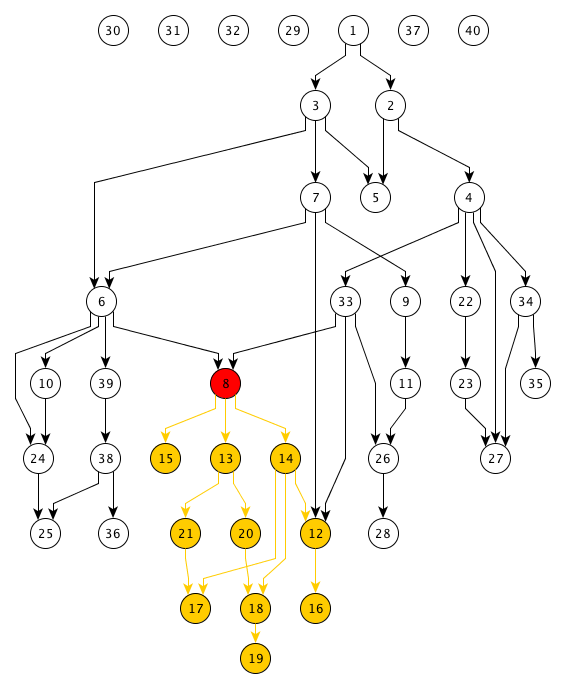
\includegraphics[scale=0.3]{pictures/subgraph_extraction_algorithm_step_2.png}
}
\caption{Sub-graph extraction from the Gene Ontology}
\end{figure}

\item Interactively select node in the Gene Ontology graph (Figure~\ref{fig:step_1}).

\item When node is selected the program computes all successors (Figure~\ref{fig:step_2}).

\item Extract leafs from successors (Figure~\ref{fig:step_3}).

\begin{figure}[h!]
\centering
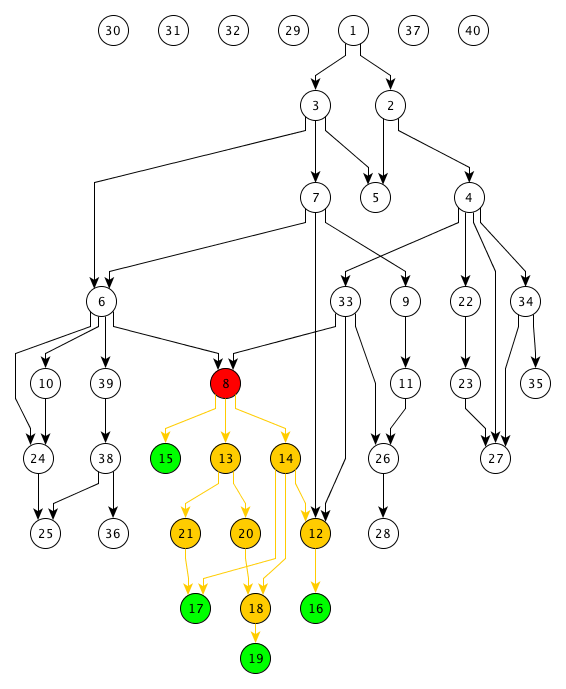
\includegraphics[scale=0.5]{pictures/subgraph_extraction_algorithm_step_3.png}
\caption{Extract leafs from the Gene Ontology sub-graph}
\label{fig:step_3}
\end{figure}

\item On this step program finds sub tree and caches. This sub tree is highlighted in cluster analysis tree.

\item The program searches corresponded leaves in cluster analysis result tree by label, as showed in Figure~\ref{fig:step_4}.

\item For any item the program finds root connected to all leaves and extracts corresponding sub trees (Figure~\ref{fig:step_5}).
\end{enumerate}

\begin{figure}[h!]
\centering
\subfloat[Find corresponded leafs]{
    \label{fig:step_4}
    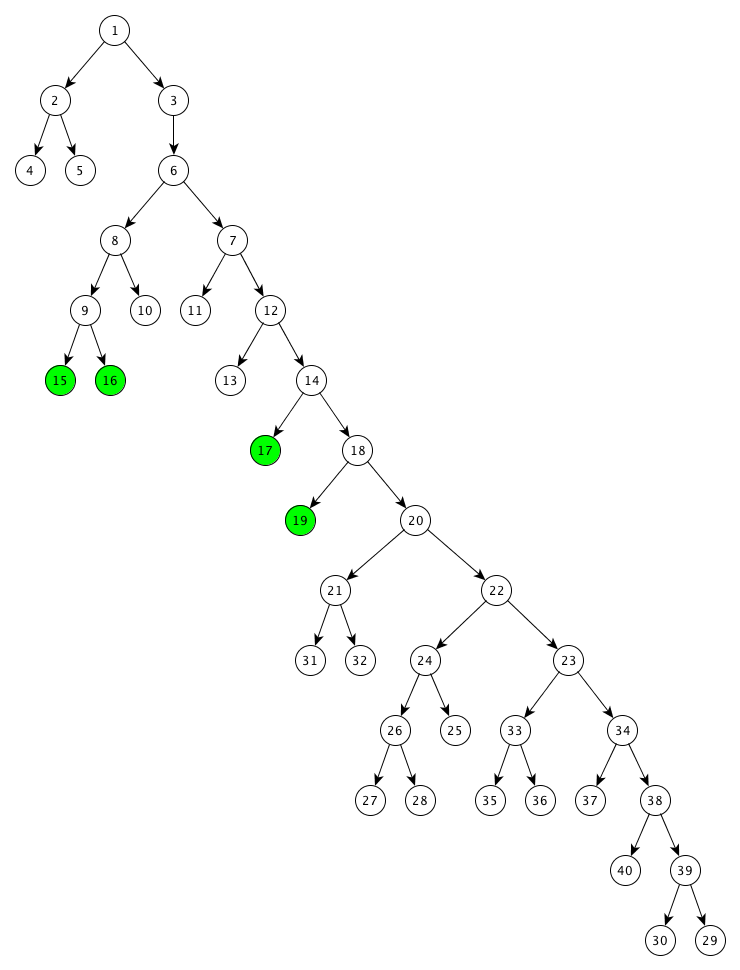
\includegraphics[scale=0.23]{pictures/subgraph_extraction_algorithm_step_4.png}
}
\subfloat[Build sub-graph]{
    \label{fig:step_5}
    
    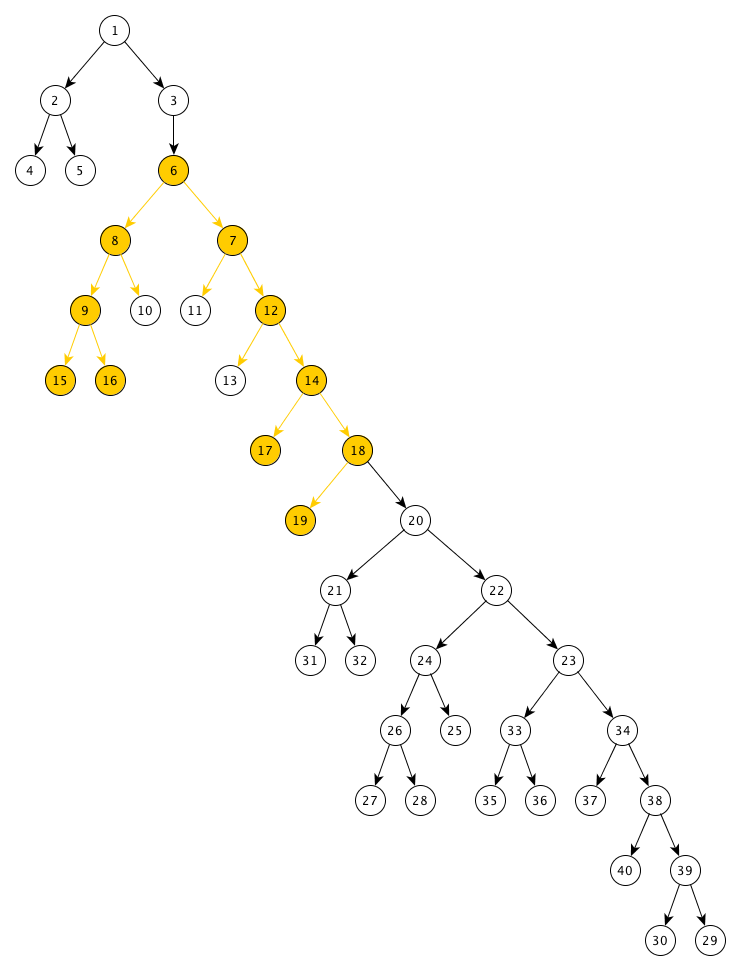
\includegraphics[scale=0.23]{pictures/subgraph_extraction_algorithm_step_5.png}
}
\caption{Analyze Cluster graph}
\end{figure}


As was mentioned before, the aim of the work is to provide flexible tool specially made for biology scientists to deal with huge data sets.
To trace relations in the two separated datasets (Gene Ontology graph and cluster analysis result tree): both graphs are stored separately in the different files.
Also during program design we had to consider that cluster analysis results graph was produced from Gene Ontology graph using separate tool and clustering algorithm specific to the purpose.
This means that there are various cluster graphs for the same Gene Ontology.

The tools provides effective space filling visualization method and allows interactive relations highlighting.
The tool also provides ability to track graphs discovering: focused or selected vertex and label are showed for both graphs separately.

Considering end-user requirements there is a use case specification for biology scientist --
interest in the concrete gene in the Gene Ontology. Also scientists are interested in the search mechanism to find specific gene by name and view it immediately on the graph.

\section{Visualization Approach}
\label{sec:solution}

\subsection{Clustering Visualization -- First Attempt}
\label{sec:probe}

As was discussed before in Section~\ref{sec:dataset_description} cluster analysis result graph is binary tree.

,,A binary tree is a connected acyclic graph such that the degree of each vertex is no more than 3. A rooted binary tree is such a graph that has one of its vertices of degree no more than 2 singled out as the root. With the root thus chosen, each vertex will have a uniquely defined parent, and up to two children; however, so far there is insufficient information to distinguish a left or right child. If we drop the connectedness requirement, allowing multiple connected component in the graph, we call such a structure a forest''~\cite{BINARY_TREE} A simple binary tree is shown in Figure~\ref{fig:simple_binary_tree}

\begin{figure}[h!]
\centering
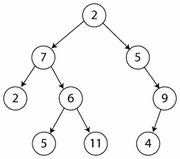
\includegraphics[scale=1.0]{pictures/simple_binary_tree.png}
\caption{A simple binary tree graph}
\label{fig:simple_binary_tree}
\end{figure}

There are several visualization methods for binary trees and more specific methods for cluster results. The main method for visualizing clusters is a dendrogram. Here is sample dendrogram visualization in Figure~\ref{fig:dendrogram_1} produced by MATLAB 7.2.

\begin{figure}[h!]
\centering
\subfloat[Dendrogram]{
    \label{fig:dendrogram_1}
    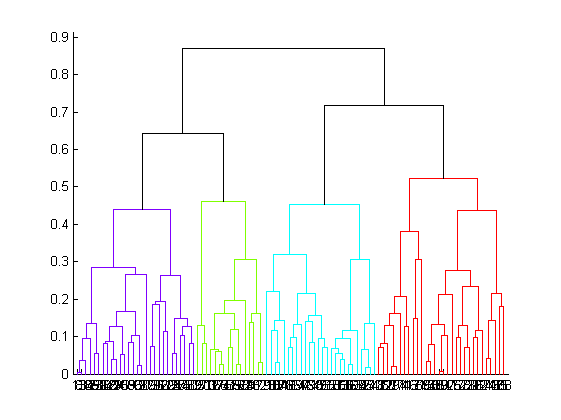
\includegraphics[scale=0.45]{pictures/dendrogram.png}
}
\subfloat[Polar Dendrogram]{
    \label{fig:polardendrogram}
    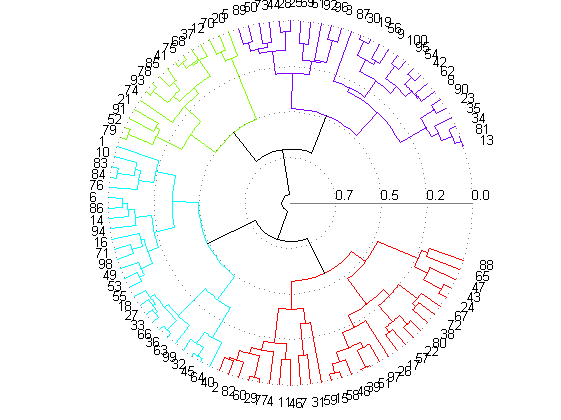
\includegraphics[scale=0.45]{pictures/polardendrogram.png}
}
\label{fig:dendrograms}
\caption{Cluster visualisations}
\end{figure}


Figure~\ref{fig:polardendrogram} shows a polar dendrogram visualization algorithm of the same cluster tree produced by MATLAB.

One of the main ideas was to use a polar dendrogram algorithm for cluster visualization. Figure~\ref{fig:JUNG_radial_layout} shows visualization of the Cluster using native JUNG radial layout algorithm. Red are nodes and white is edges, black is background. As picture shows algorithm doesn't count nature of the cluster: very deep binary tree not wide as it is common for cluster analysis results, that's why it has many edge overlapping.


\begin{figure}[h!]
\centering
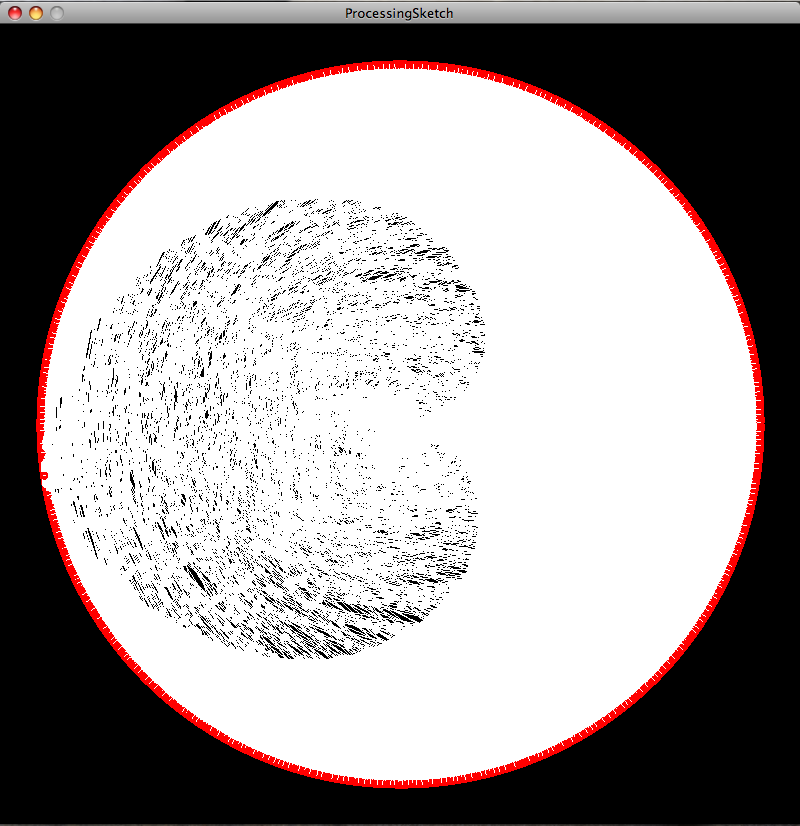
\includegraphics[scale=0.4]{pictures/using_JUNG_radial.png}
\caption{Cluster visualization using JUNG radial layout}
\label{fig:JUNG_radial_layout}
\end{figure}


Also to visualization issue it has performance issue -- without any measurement was seen for an eye that program does not allow smooth interaction. Low performance issue was in nature of the visualization in the JUNG: it uses very complex hierarchical structure with many utility classes per visualized object and the cost is big memory usage. Also JUNG uses Java 2D~\cite{JAVA_2D} which by itself is `heavyweight' because it's part of the Java AWT -- Abstract Windows Toolkit.


,,The Abstract Window Toolkit (AWT) is Java's original platform-independent windowing, graphics, and user-interface widget toolkit. The AWT is now part of the Java Foundation Classes (JFC) the standard API for providing a graphical user interface (GUI) for a Java program. When Sun Microsystems first released Java in 1995, AWT widgets provided a thin level of abstraction over the underlying native user interface. For example, creating an AWT check box would cause AWT directly to call the underlying native subroutine that created a check box.''~\cite{JAVA_AWT} This technology is outdated and replaced by Swing.


,,Swing is the primary Java GUI widget toolkit. It is part of Sun Microsystems' Java Foundation Classes (JFC) an API for providing a graphical user interface (GUI) for Java programs.
Swing was developed to provide a more sophisticated set of GUI components than the earlier Abstract Window Toolkit. Swing provides a native look and feel that emulates the look and feel of several platforms, and also supports a pluggable look and feel that allows applications to have a look and feel unrelated to the underlying platform.''~\cite{JAVA_SWING}


,,Since early versions of Java, a portion of the Abstract Window Toolkit (AWT) has provided platform-independent APIs for user interface components. In AWT, each component is rendered and controlled by a native peer component specific to the underlying windowing system.
By contrast, Swing components are often described as lightweight because they do not require allocation of native resources in the operating system's windowing toolkit. The AWT components are referred to as heavyweight components.''~\cite{JAVA_SWING} More detail comparison can be found here.~\cite{AWT_VS_SWING}


Figure~\ref{fig:cluster_jogl_impl} shows improved JUNG radial algorithm and own visualization implementation using JOGL will be discussed in Section~\ref{sec:opengl}..

Root has fixed position in the center of the ring. The layout places all leafs evenly on the outer ring based on the distance from root. Each node is placed on the concentric ring corresponding to its distance to the root node -- level. Each node is radially centered over children. The number of concentric rings is exactly equal to the number of levels of the graph.


\begin{figure}[h!]
\centering

\includegraphics[scale=0.4]{pictures/cluster_jogl_impl.png}
\caption{Cluster visualization using JOGL and improved JUNG radial layout}
\label{fig:cluster_jogl_impl}
\end{figure}


Figure~\ref{fig:cluster_jogl_impl_with_subgraph_1} and Figure~\ref{fig:cluster_jogl_impl_with_subgraph_2} show cluster visualization and highlighted subgraph (subgraph extraction algorithm was discussed in Section~\ref{sec:algorithm}). This pictures show the nature of the dataset. Improved version has good performance and better visualization but still has issues: there are too many elements in the scene, it is impossible to identify separate gene or trace highlighted graph genes.

\begin{figure}[h!]
\centering
\subfloat[Cluster graph and highlighted subgraph]{
    
\includegraphics[scale=0.2]{pictures/cluster_jogl_impl_with_subgraph_1.png}
    \label{fig:cluster_jogl_impl_with_subgraph_1}
}
\subfloat[Cluster graph and highlighted subgraph]{
    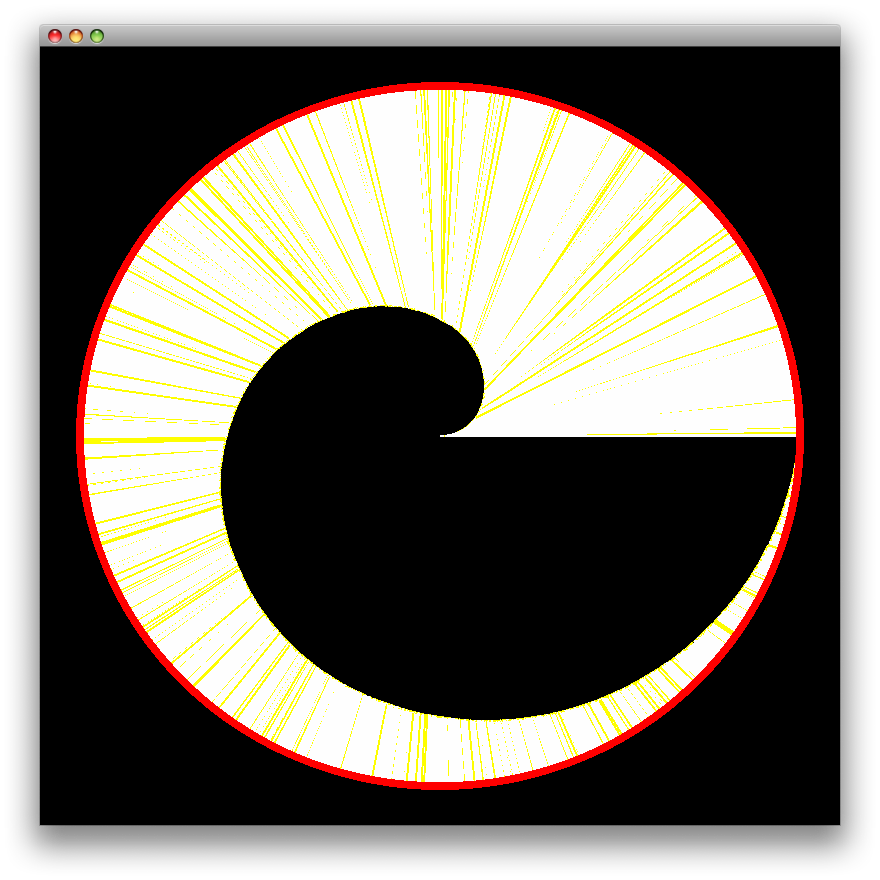
\includegraphics[scale=0.2]{pictures/cluster_jogl_impl_with_subgraph_2.png}
    \label{fig:cluster_jogl_impl_with_subgraph_2}
}
\caption{Cluster graph visualization using improved JUNG polar dendrogram layout}
\end{figure}


%%%%%%%%%%%%%%%%%%%%%%%%%%%%%%%%%%%%%%%%%%%%%%%%%%%%%%%%%%%%%%%%%%%%%%%%%%%%%%%%%%%%%%%%%%%%%%%%%%%%
% cluster visualization explanation
\subsection{Cluster Analysis Results Visualization}
\label{sec:cluster}

Figure~\ref{fig:Cytoscape_Cluster_2} from Section~\ref{sec:dataset_description} shows cluster graph specific structure: it is very high, unbalanced and has not so deep sub-parts. It is possible to use this disadvantage as advantage and abstract sub-parts to reduce drawing area. Extract those nodes and edges that form the longest path of the cluster graph - ,,backbone''. Figure~\ref{fig:cluster_visualisation} shows algorithm work step by step. Backbone vertices are filled with yellow and showed in Figure~\ref{fig:cluster_visualisation_algorithm_1}. Next step is to abstract branches into groups, group size is scaled according to amount of elements inside.

\begin{figure}[h!]
\centering
\subfloat[Backbone and branches]{
    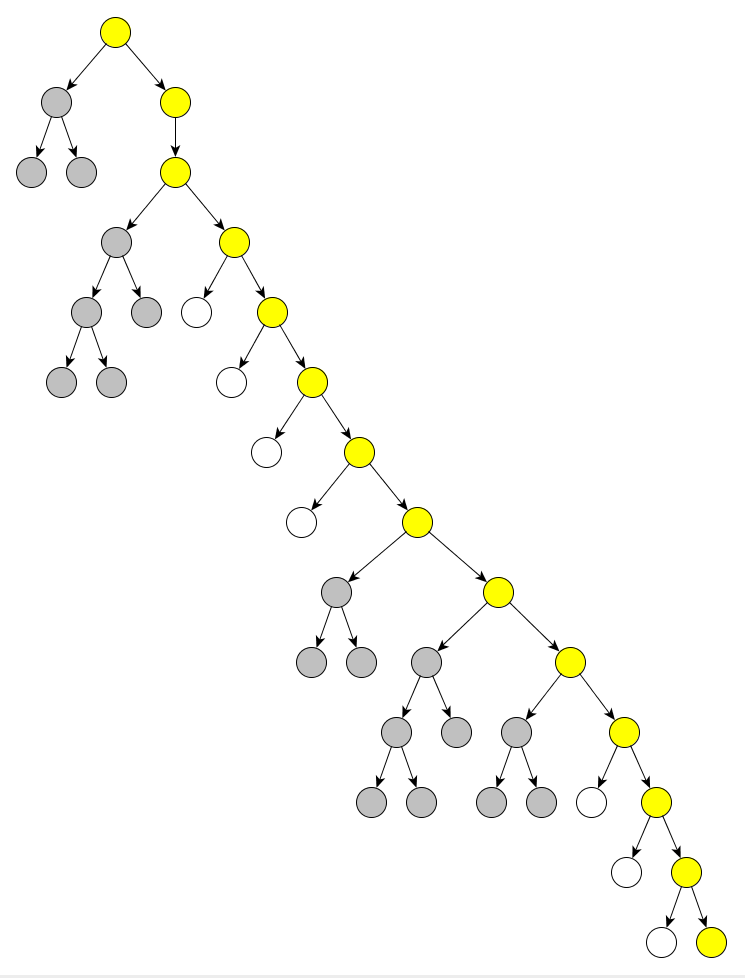
\includegraphics[scale=0.15]{pictures/cluster_visualisation_algorithm_1.png}
    \label{fig:cluster_visualisation_algorithm_1}
}
\subfloat[Abstract branches into groups]{
    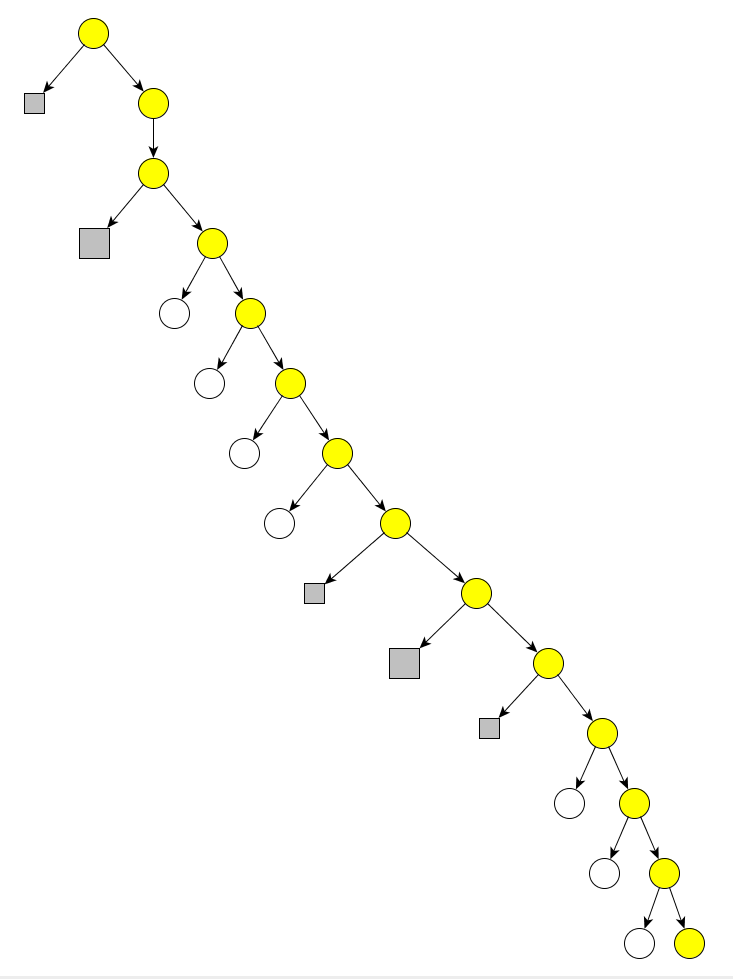
\includegraphics[scale=0.15]{pictures/cluster_visualisation_algorithm_2.png}
    \label{fig:cluster_visualisation_algorithm_2}
}
\subfloat[Scale group size]{
    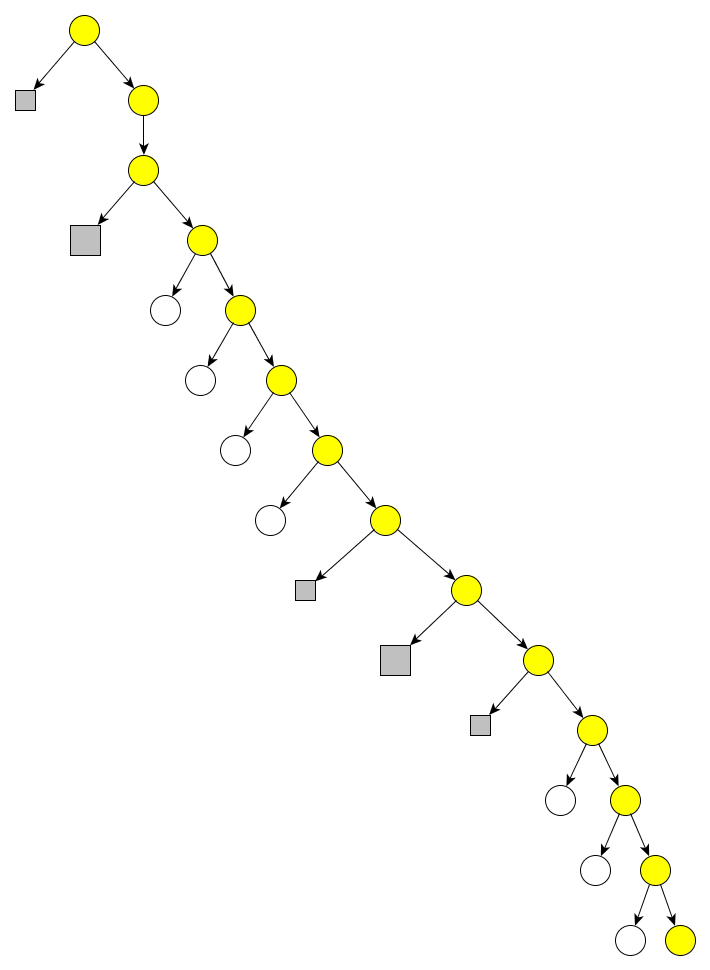
\includegraphics[scale=0.15]{pictures/cluster_visualisation_algorithm_3.png}
    \label{fig:cluster_visualisation_algorithm_3}
}
\caption{Cluster Visualization algorithm}
\label{fig:cluster_visualisation_algorithm}
\end{figure}

The last step is to represent backbone as a spiral, thus preserving space and giving us a possibility to show the complete tree in one view. Figure~\ref{fig:cluster_visualisation_algorithm_4} shows how this approach works.

\begin{figure}[h!]
\centering
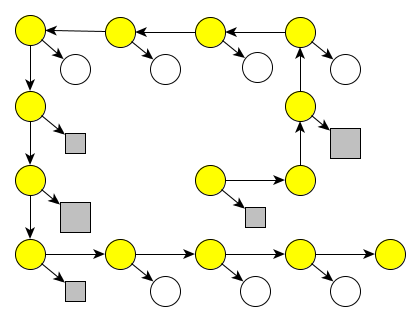
\includegraphics[scale=0.5]{pictures/cluster_visualisation_algorithm_4.png}
\caption{,,Rectangular Spiral Layout''}
\label{fig:cluster_visualisation_algorithm_4}
\end{figure}

Then backbone formed as rectangular spiral with a root in the center and moving in clockwise direction. Figure~\ref{fig:cluster_spiral_visualisation} shows complete visualization result for real cluster tree. This will have to reuse space as much as possible and still gives overview of location of the highlighted vertices in cluster hierarchy -- how far from a root.

\begin{figure}[h!]
\centering
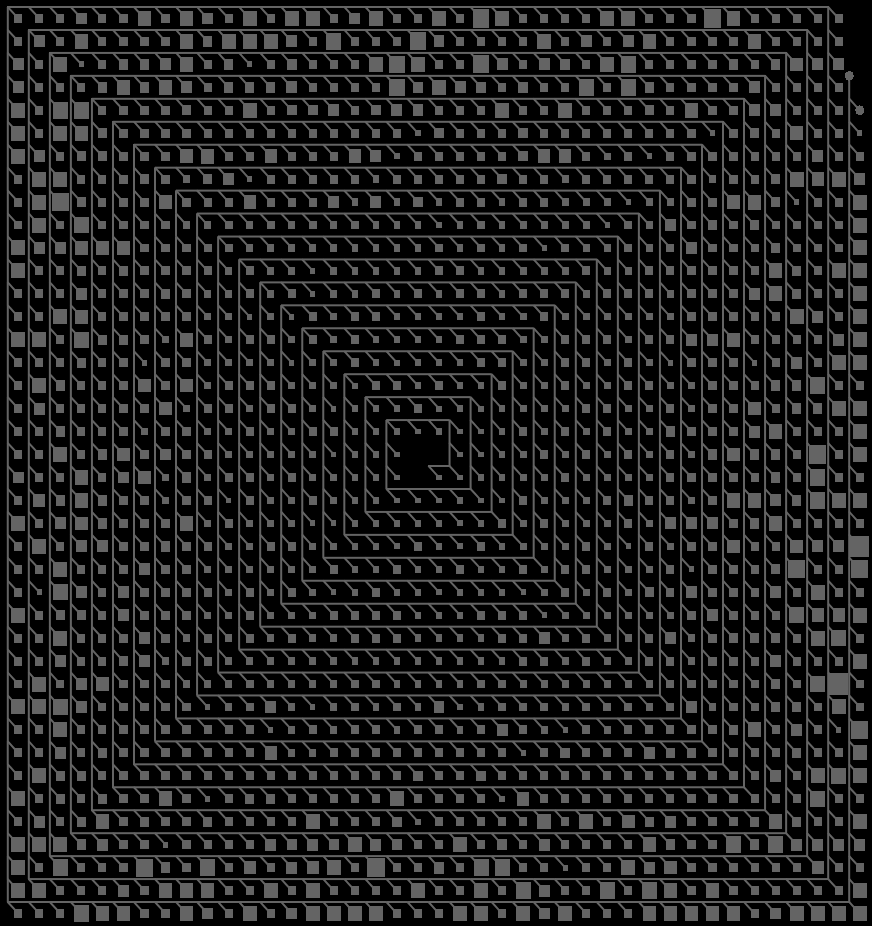
\includegraphics[scale=0.4]{pictures/cluster_spiral_visualisation.png}
\caption{Rectangular spiral Cluster graph visualization}
\label{fig:cluster_visualisation}
\end{figure}

It is possible to explore sub-part (rectangles) of the Cluster graph using lens. User can interactively choose any sub-part and lens with inner content will appear. There are two different lens layouts: polar~\ref{fig:lens_polar} and HV-tree~\ref{fig:lens_tree}. Polar lens layout is based on algorithm used for initial visualization of the Cluster graph explained earlier in Section~\ref{sec:probe}. Both implementations are own made and are not based on any third party source code.

\begin{figure}[h!]
\centering
\subfloat[Polar lens layout]{
    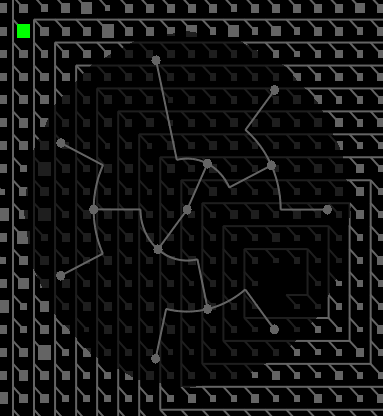
\includegraphics[scale=0.5]{pictures/lens_polar.png}
    \label{fig:lens_polar}
}
\\
\subfloat[HV-tree lens layout]{
    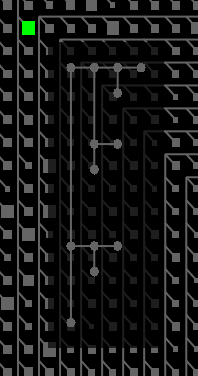
\includegraphics[scale=0.5]{pictures/lens_tree.png}
    \label{fig:lens_tree}
}
\caption{Different lens layouts}
\end{figure}


%%%%%%%%%%%%%%%%%%%%%%%%%%%%%%%%%%%%%%%%%%%%%%%%%%%%%%%%%%%%%%%%%%%%%%%%%%%%%%%%%%%%%%%%%%%%%%%%%%%%


%%%%%%%%%%%%%%%%%%%%%%%%%%%%%%%%%%%%%%%%%%%%%%%%%%%%%%%%%%%%%%%%%%%%%%%%%%%%%%%%%%%%%%%%%%%%%%%%%%%%
% gene ontology visualization explanation
\subsection{Gene Ontology Visualization}
\label{sec:go}

Gene Ontology graph is a directed acyclic graph and highly connected: 24,153 edges and 10,041 vertices, where 3,918 are unconnected components.
Figure~\ref{fig:go_connections_yEd} shows how extremely connected the graph is, the picture was produced by yEd graph editing tool.

\begin{figure}
\centering
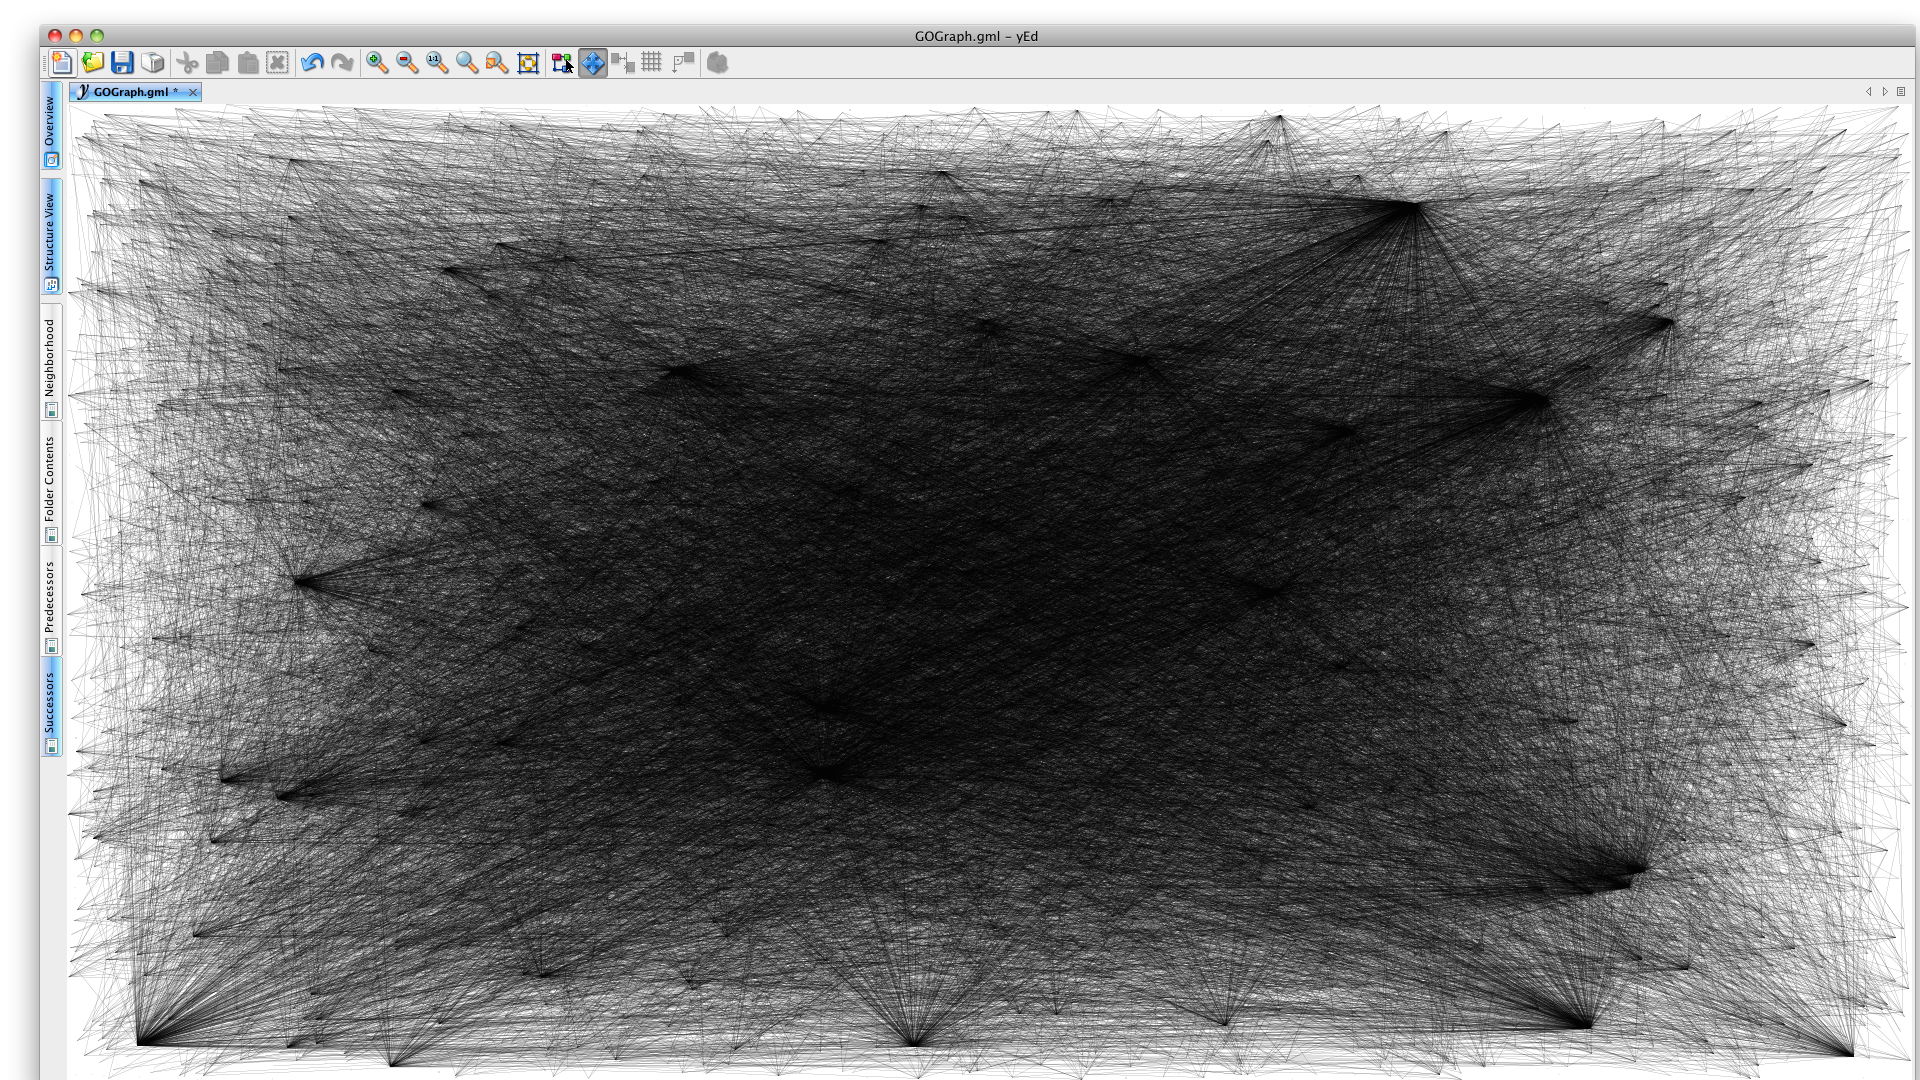
\includegraphics[scale=0.2]{pictures/yEd_GO_2.png}
\caption{Gene Ontology graph visualization using yEd}
\label{fig:go_connections_yEd}
\end{figure}

The high connectivity between elements in the source graph makes it very complicated to explore. Provided visualization approach has several goals.
The first goal is to reduce amount of connections between vertices by showing edges only for ``current'' sub-graph.
It allows to see where the sub-graph is aligned in the whole graph and, in the same time, helps to track its inner structure.
Second goal is an ability to switch from working with genes of the GO graph to discovering relations between GO and Cluster graphs.
For this purpose there are two view modes for GO graph:

\begin{itemize}
   \item levels overview --- show graph levels from top to bottom with corresponding content as ``preview'';
   \item zoomed view --- visualizes only on three levels at the same time in order to focus on genes inside;
\end{itemize}

The last but not least goal is to explicitly show nodes and leafs. Each level is divided into two sections where leafs are red colored on the left and node genes are on the right and having white color.
Color schema can be changes through the settings menu but not leafs-nodes location.
This feature gives further insight into the topology of a specific layer by gaining information about the distribution of leafs and nodes on a particular layer.

There are two layout implementations based on the goals discussed before. First GO layout is ``Levels Layout'' and is shown in Figure~\ref{fig:go_levels_layout}.
Genes are ordered by layers depending on their graph-theoretic distance from the root.

\begin{figure}[h!]
\centering
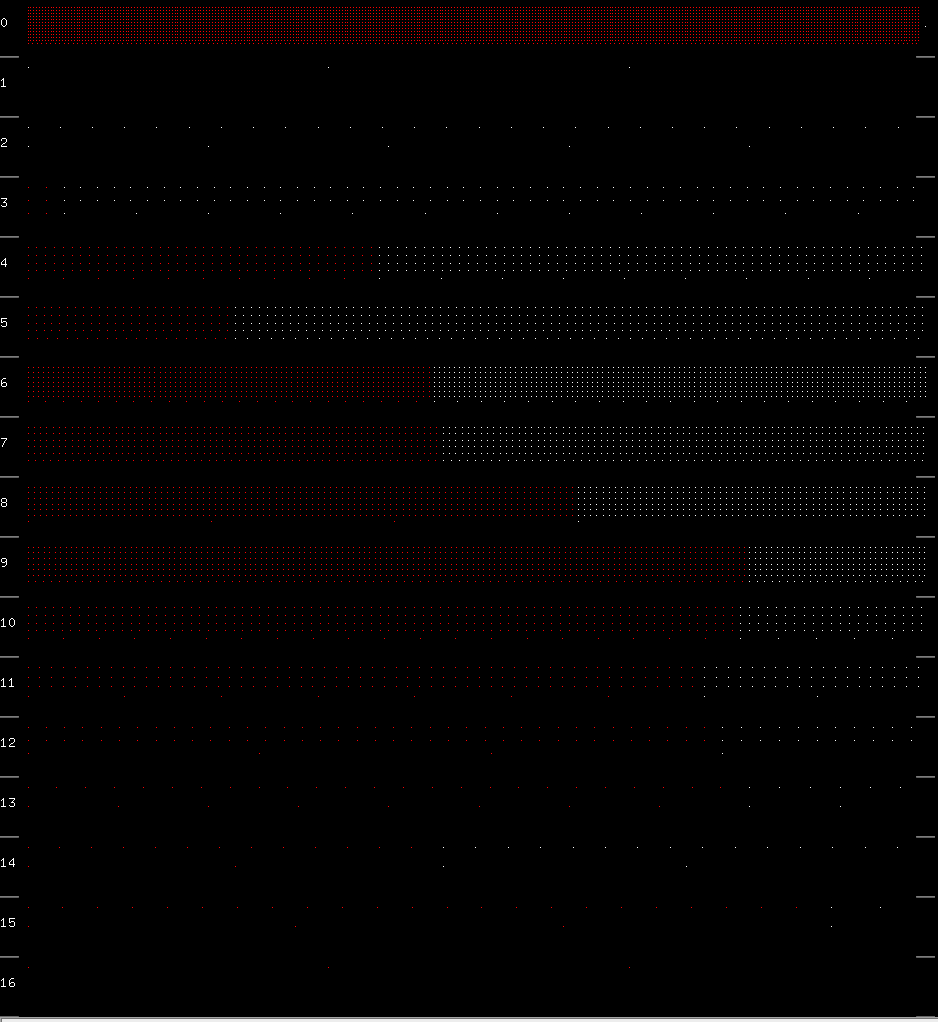
\includegraphics[scale=0.3]{pictures/go_levels_layout.png}
\caption{Gene Ontology Levels Layout visualisation}
\label{fig:go_levels_layout}
\end{figure}

Figure~\ref{fig:go_levels_layout_zoomed} displays the situation when the user zooms in the view.
Although the resulting visualization looks like bar charts, the number of leafs cannot be precisely compared between different layers since
the area the red node pixels (leafs) cover is not proportional to the total number of leafs in each layer.
However, it is proportional to the sum of nodes in that particular layer. In other words, the covered area depends on the specific layer density.
There are unconnected components in the Gene Ontology graph.
Unconnected nodes are placed in the top layer number --- zero. There is an option to show-hide unconnected components from the main menu.
The spatial arrangement of the node pixels within a layer, except the placing of leafs and nodes are in specific regions, is random.

\begin{figure}[h!]
\centering
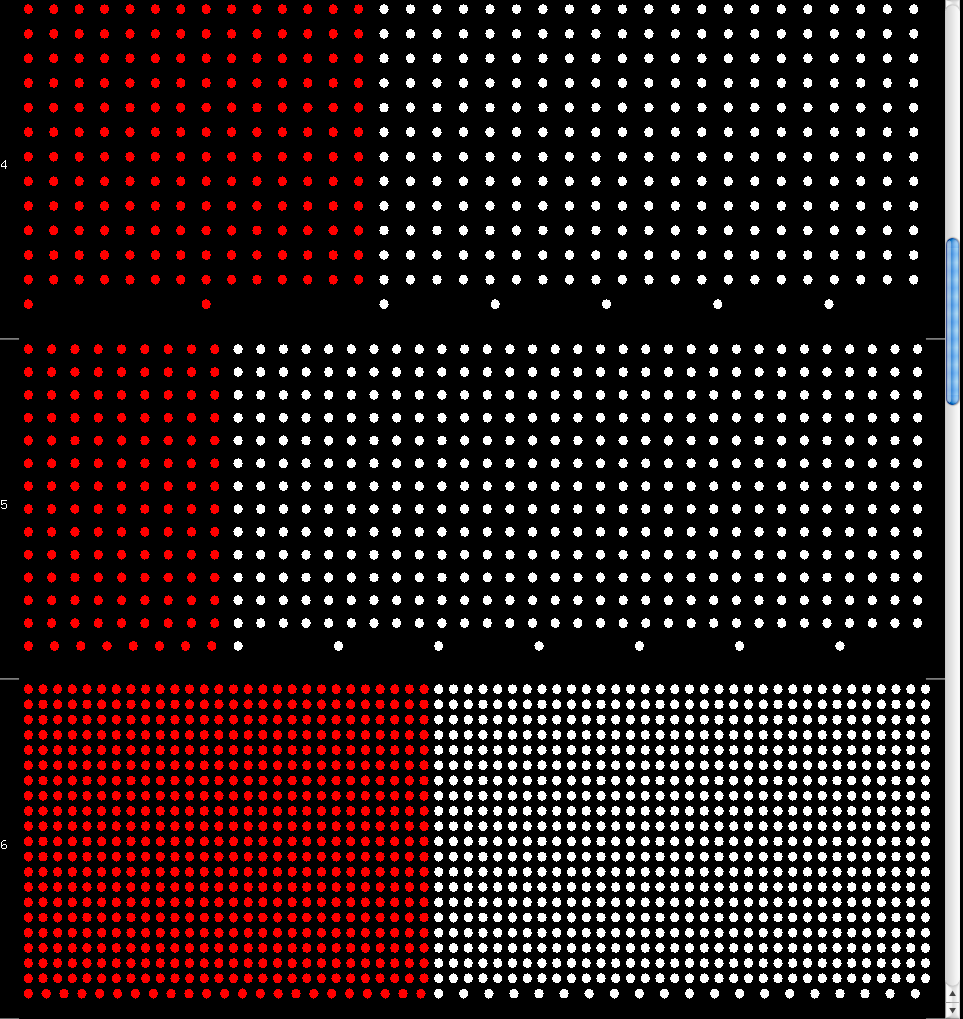
\includegraphics[scale=0.3]{pictures/go_levels_layout_zoomed.png}
\caption{Zoomed view}
\label{fig:go_levels_layout_zoomed}
\end{figure}

Second layering approach ``Leaves Bottom Layout''
(Figure~\ref{fig:go_leaves_bottom_layout}) is similar to the first one in terms of placing the nodes into corresponding layers based on the distance
from the source node and random distribution of the node pixels within each layer.
However, all leafs are placed into one single layer together with unconnected nodes at the bottom of the GO view, i. e., in the layer with the highest number.
Unconnected nodes can be filtered out if necessary. This approach gives insight into the distribution of nodes among different layers without the distraction of the leafs,
thus enriching the perception of the graph topology.

\begin{figure}[h!]
\centering
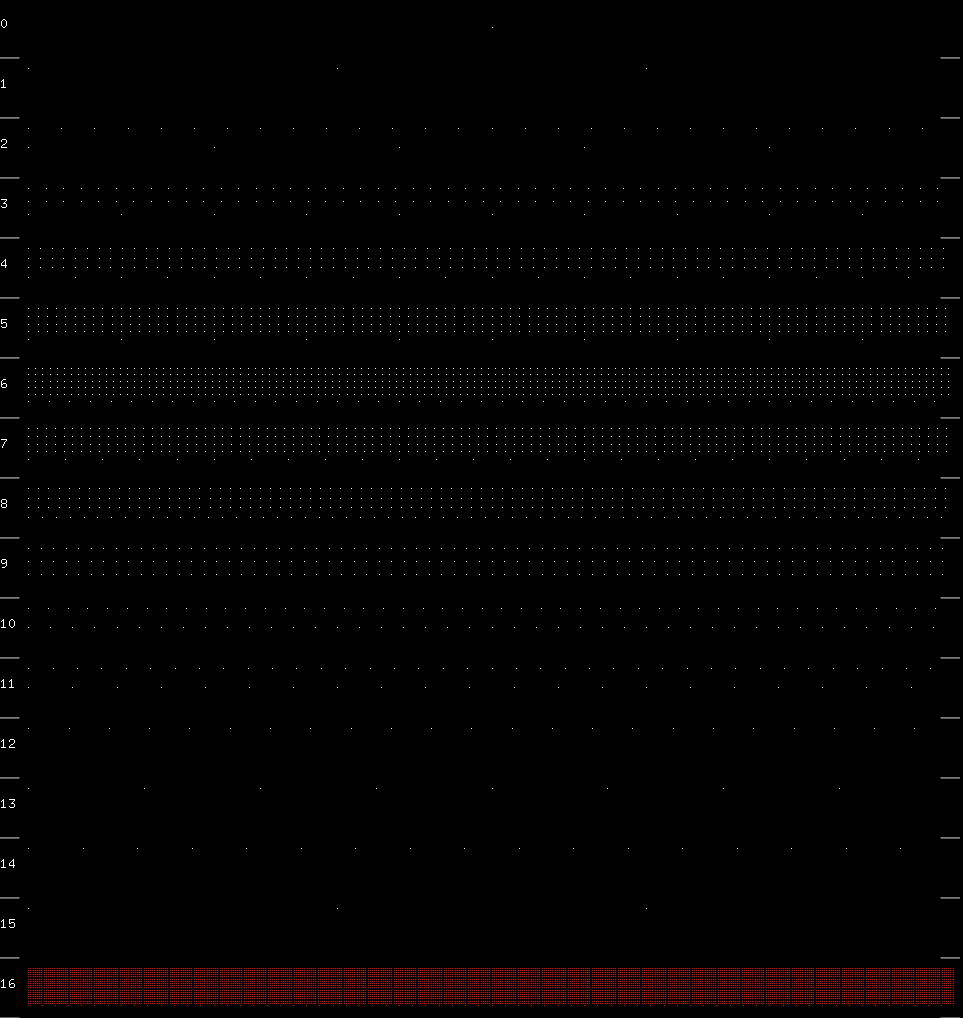
\includegraphics[scale=0.3]{pictures/go_leaves_bottom_layout.png}
\caption{Leaves bottom layout}
\label{fig:go_leaves_bottom_layout}
\end{figure}

All provided features help to improve visualization and decrees amount of element in the scene. But even with hided edges visualized sub-tree could be complicated.
The result of sub-graph highlighting is shown in Figure~\ref{fig:go_no_edge_bundling}.

\begin{figure}[h!]
\centering
\subfloat[Straight edges]{
    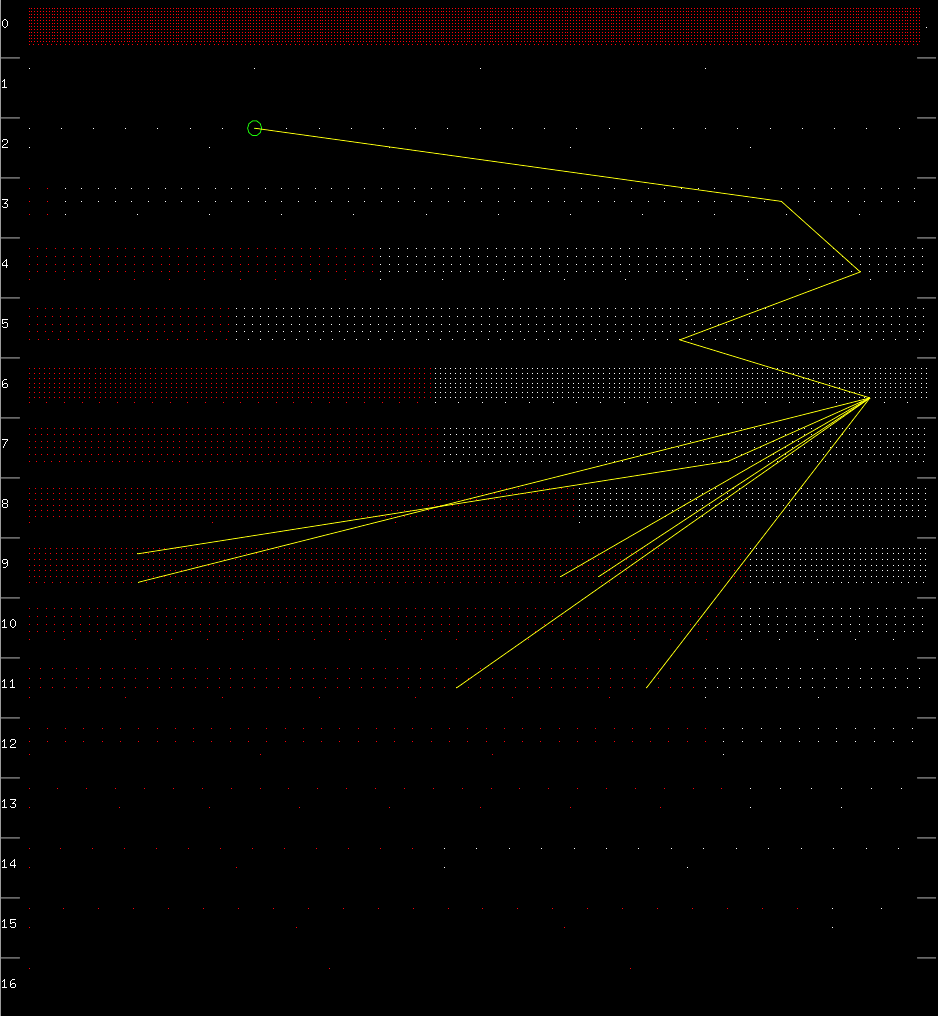
\includegraphics[scale=0.2]{pictures/go_no_edge_bundling.png}
    \label{fig:go_no_edge_bundling}
}
\subfloat[Edge bungling]{
    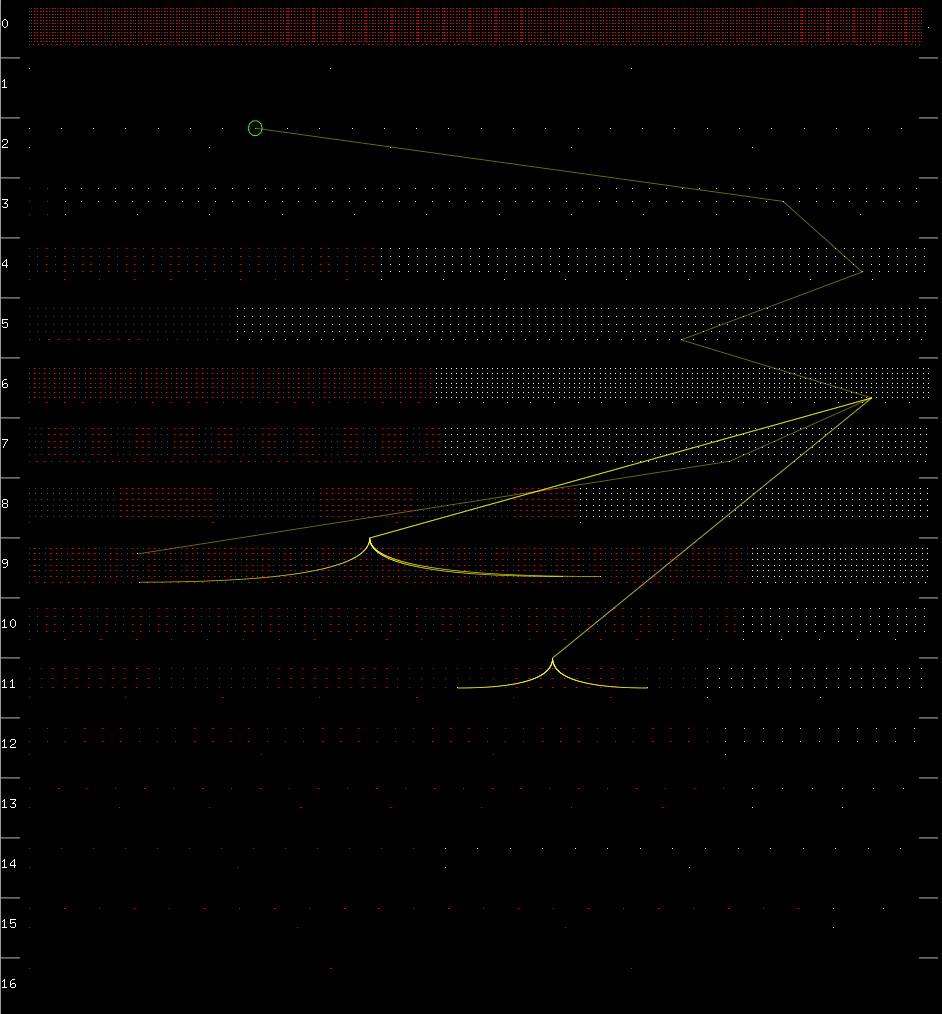
\includegraphics[scale=0.2]{pictures/go_edge_bundling.png}
    \label{fig:go_edge_bundling}
}
\caption{Gene Ontology sub-graph edge highlighting}
\label{fig:go_subgraph_highlighting}
\end{figure}

Improved edge visualization for the same selected vertex ``multicellular organismal process'' is shown in Figure~\ref{fig:go_edge_bundling}.
A newer solution is simple edge bundling. Edge bundling technique and usage example well described in the~\cite{EDGE_BUNDLING_1} and~\cite{EDGE_BUNDLING_2}.

For all edges which go into same level computed ``dummy node'' located on the top of the target level and in the middle of outlined vertices, drawing single line from source to
``dummy node'' as first part. Second part is to draw ``Bezier line'' from ``dummy node'' to target vertex. This solution helps to follow the connection and to use space in the right way.
%%%%%%%%%%%%%%%%%%%%%%%%%%%%%%%%%%%%%%%%%%%%%%%%%%%%%%%%%%%%%%%%%%%%%%%%%%%%%%%%%%%%%%%%%%%%%%%%%%%%

\subsection{Complete Solution Overview}
\label{sec:complete_solution_overview}

Biologists usually browse the data set randomly, or have a specific GO term in mind. For that purpose it is possible either search for specific gene in a list that is shown in the dialog box called from the menu, or directly click on a particular node in the GO view. A mouse-over action on a node will display the name of that node with the help of a tool-tip. This helps the user to browse the GO and to select a node for further exploration. The GO view displays the nodes as single pixels as already explained earlier. It is pretty hard to perceive a single selected pixel by using color coding only. To make this task easier there is a green circle around the selected node in the GO view, as seen in the third layer of the GO view in Figure~\ref{fig:complete_solution_overview}. This feature makes it also easier to identify the layer the currently selected node belongs to. After the node has been selected by clicking, the sub-graph consisting of all reachable nodes will be calculated. These related nodes, as explained in Subsection~\ref{sec:go}, will be highlighted in yellow in the both views. Optionally, the edges of the sub-graph will be shown too. At the same time, the corresponding cluster sub-tree will be highlighted with the same color in the Cluster Tree view reflecting the selection made in the GO view. In this way, the user can easily identify the mapping between both views by comparing the highlighted elements. Note that the closer the selected node is to the GO root, the larger the number of nodes can be accessed from that particular node. For example, the root node of the GO DAG has access to all nodes of the DAG, this means that if the root node pixel is clicked, the complete DAG is selected. In such cases, clutter cannot be avoided. Therefore, users can choose the option to disable the visualization of edges if needed to reduce information overloading. More screen shots can be found in the Appendix~D.

\begin{figure}[h!]
\centering
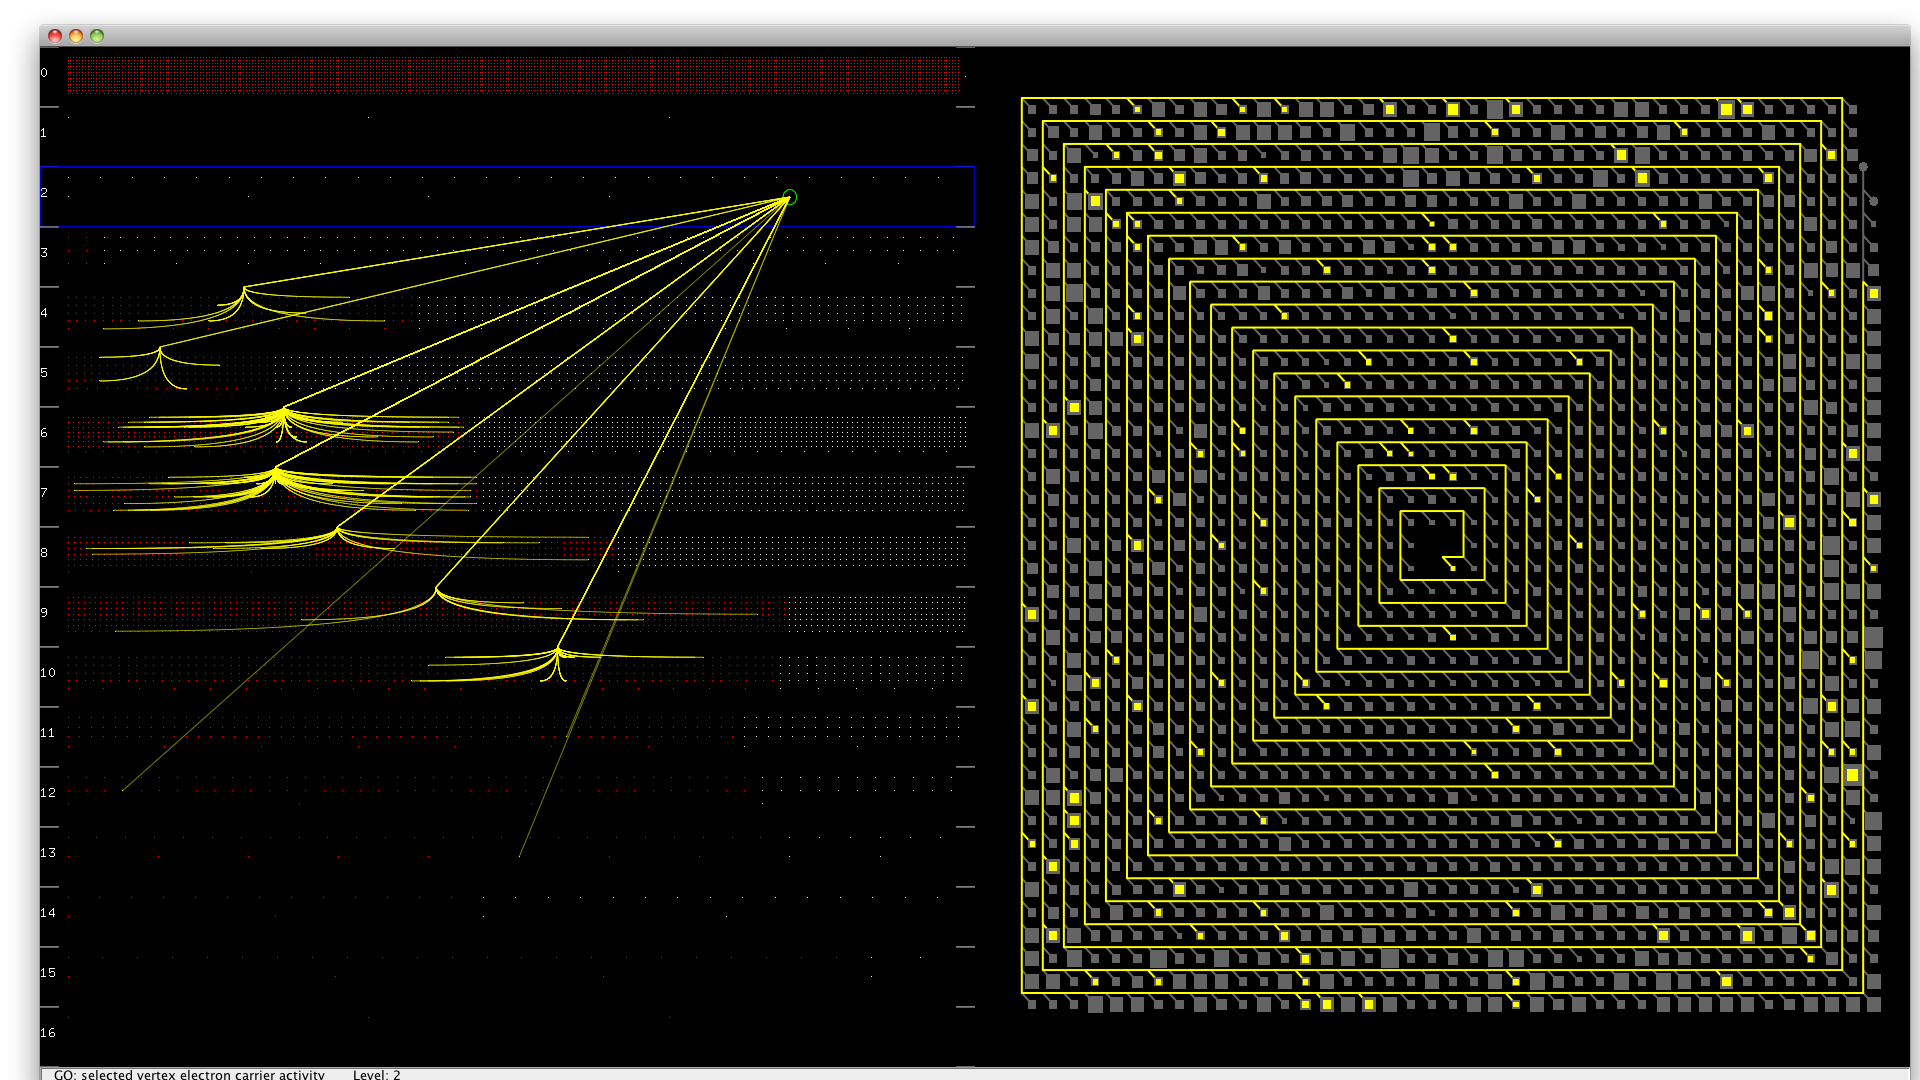
\includegraphics[scale=0.33, angle=90]{pictures/complete_solution_overview.png}
\caption{The result of the complete visualization solution with interaction technique}
\label{fig:complete_solution_overview}
\end{figure}


\mysection{Implementation}{sec:implementation}

Current section covers technical details of the implementations of the tool. It covers module abstractions of the system, overview of the tools that were used during the development and
short discussions about the reasons as well.

\subsection{Programming Language and Tools}

Main language and platform for developing thesis is Java. Java is a programming language and computing
platform first released by Sun Microsystems in 1995. It is the underlying technology that powers state-of-the-art
programs including utilities, games, and business applications. Java runs on more than 850 million personal computers worldwide,
and on billions of devices worldwide, including mobile and TV devices.~\cite{java_com}
Also, there are a lot of different libraries in Java. Every common part of the system could be replaceable.
In the future sections would be detailed overview libraries for graphs, graph visualizations and graphic libraries.


Java is flexible platform which has big amount of different libraries. It helps not to write twice things already made but flexibility cause project structure complexity and library management. On the early stage there are no problems to control project throw sophisticated IDE (integrated development environment) but as project complexity grows more powerful building tool need appears. Maven is used during thesis work.


Maven~\cite{MAVEN_HOME_PAGE} is free, open-source and de-facto project management standard on the Java platform,
is part of Apache software project developed and supported by ASF (Apache Software Foundation)~\cite{APACHE_FOUNDATION_HOME_PAGE}.

\begin{quotation}
``Maven provides a comprehensive approach to managing software projects.
From compilation, to distribution, to documentation, to team collaboration,
Maven provides the necessary abstractions that encourage reuse and take much of the work out of project builds.''~\cite{MAVEN_BOOK_1}
\end{quotation}

Maven is a set of standards, a repository format, and a piece of software used to manage and describe projects.
It defines a standard life cycle for building, testing, and deploying project artifacts.
It provides a framework that enables easy reuse of common build logic for all projects following Maven's standards.
The Maven project at the Apache Software Foundation is an open source community which produces software tools that
understand a common declarative Project Object Model (POM).~\cite{MAVEN_BOOK_2}


Maven's primary goal is to allow a developer to comprehend the complete state of a development effort in the shortest period of time. In order to attain this goal there are several areas of concern that Maven attempts to deal with:
\begin{itemize}
	\item making the build process easy
	\item providing a uniform build system
	\item providing quality project information
	\item providing guidelines for best practices development
	\item allowing transparent migration to new features
\end{itemize}


In Figure~\ref{fig:THESIS_FOLDER_STRUCTURE} is the structure of the project folder. Thesis project uses standard Maven project folder format. Here is overview of key parts: java source code stored in the ``src/main/java'' folder, tests source code stored in the ``src/test/java''. Necessary resources such as log4j configuration file stored in the ``src/main/resources'', in the same folder thesis properties file is stored. During ``package'' phase all resources are copied by Maven.


``Native'' directory stores JOGL native libraries to different platform such as Linux, Windows and Mac OS X. In the ``lib.zip'' stored jars for JUNG library which should be manually placed in the local Maven repository because they do not  exist in central Maven repository. All other dependencies are exist in Maven repositories and handled by default dependency process.


Complete builds are stored in the ``build'' folder. Latest build stored in the ``build/latest'' folder, other builds stored in the folder that has such name pattern:


\texttt{GoClusterViz-\%version\%-\%build date\%-\%build time\%}


Each build folder contains corresponded native build for each of three platforms Linux, Windows and Mac OS X. Cluster graph and Gene Ontology graphs are stored in the ``data'' folder.

\begin{figure}[h!]
\centering
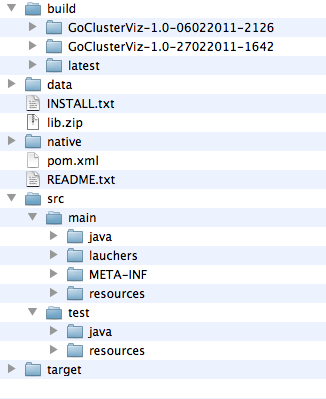
\includegraphics[scale=0.7]{pictures/thesis_folder_structure.png}
\caption{Thesis folder structure}
\label{fig:THESIS_FOLDER_STRUCTURE}
\end{figure}

Second necessary part of the normal development process is revision control.

\begin{quotation}
``Revision control, also known as version control or source control (and an aspect of software configuration management or SCM),
is the management of changes to documents, programs, and other information stored as computer files.
It is most commonly used in software development, where a team of people may change the same files.
Changes are usually identified by a number or letter code, termed the `revision number', `revision level', or simply `revision'.
For example, an initial set of files is `revision 1'. When the first change is made, the resulting set is `revision 2', and so on.
Each revision is associated with a time stamp and the person making the change. Revisions can be compared,
restored, and with some types of files, merged.''~\cite{REVISION_CONTROL}
\end{quotation}

During thesis development Git version control system was used.

\begin{quotation}
``Git is a distributed revision control system with an emphasis on speed.
Git was initially designed and developed by Linus Torvalds for Linux kernel development.
Every Git working directory is a full-fledged repository with complete history and full revision tracking capabilities,
not dependent on network access or a central server. Git is free software distributed under the terms of the
GNU General Public License Version 2.''~\cite{GIT}
\end{quotation}

Git allows to store and work locally on the machine but for safety reasons all source code stored on GitHub.
GitHub is a web-based hosting service for software development projects that use the Git revision control system.
GitHub provides free hosting for open-source project. Thesis project home page on GitHub~\cite{GitHub_homepage} and Git repository URL~\cite{GitHub_repository}.

\begin{figure}[h!]
\centering
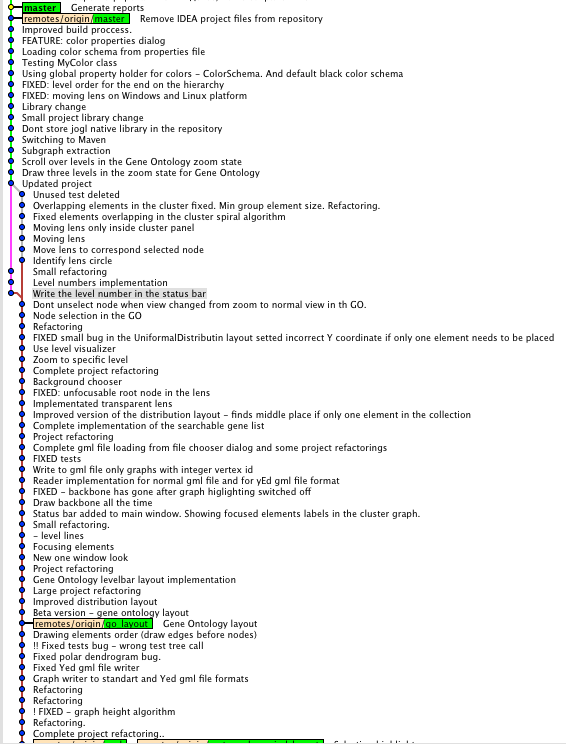
\includegraphics[scale=0.62]{pictures/commit_graph_gitk.png}
\caption{Commit graph of the local repository made by gitk tool}
\end{figure}


\subsection{Java Graph Libraries Overview}


There are overview of a few libraries for working with graphs in Java

\begin{enumerate}

\item
Java Graph Editing Framework (GEF)~\cite{GEF}

The aim of project consists in generation of library for graph editing, which can be used for construction of high-end (high-quality) custom applications for working with graphs.
GEF facilities (opportunities):
\begin{itemize}
	\item simple and clear design, which allows a developer to expand library's functionality
	\item Node-Port-Edge model of graph's presentation, which permits to perform overwhelming majority of tasks occurring in working with graphs applications
	\item future XML-based format support (SVG)
\end{itemize}

\item
ILOG JViews~\cite{ILOG_Jview}

ILOG JViews gives (grants) components, aimed for using in custom applications, and also in common with Ajax and Eclipse platform.

\item
JGraphT~\cite{JGraphT}

JGraphT is open source library, which provides with mathematical tool of graphs theory. JGraphT supports different kinds of graphs, including: oriented and unoriented graphs, graphs with weighted/non weighted/nominate (named) or anything else arc format, appointed 	by user, non upgradeable graphs - supported access to internal graphs in ``Read Only'' mode. Listenable graphs: allows outer listener to trace events appearance; sub-graphs: graphs which are a view about other graphs. Being a powerful feature, JGraphT has been 	developed as easy and type-safe (with Java code generators use) feature for working with 	graphs. For example, any object can be node of a graph. You can build graphics on basis of: line, URL, XML documents and so forth, you can even build graphs of graphs.

\item
Java Universal Network / Graph Framework (JUNG)~\cite{JUNG}

JUNG (Java Universal Network/Graph Framework) --- is a software library that provides a common utilities for the modeling, analysis, and visualization of data that can be represented as a graph or network. It is written in Java, which allows JUNG-based applications to make use of the extensive built-in capabilities of the Java API, as well as those of other existing third-party Java libraries.

\begin{quotation}
``The JUNG architecture is designed to support a variety of representations of entities and their relations,
such as directed and undirected graphs, multi-modal graphs, graphs with parallel edges, and hyper-graphs.
It provides a mechanism for annotating graphs, entities, and relations with meta data.
The current distribution of JUNG includes implementations of a number of algorithms from graph theory,
data mining, and social network analysis, such as routines for clustering, decomposition, optimization,
random graph generation, statistical analysis, and calculation of network distances, flows,
and importance measures (centrality, PageRank, HITS, etc.).''~\cite{JUNG_OVERVIEW}
\end{quotation}

JUNG library is widely used in differ amount of projects. Here is a list of projects using JUNG:

\begin{itemize}

\item ExtC: an Eclipse plug-in that is useful for locating large, non-cohesive classes and for recommending how to split them into smaller, more cohesive classes. (Keith Cassell)~\cite{EXTC}

\item Djinn: a tool for visualizing java artifacts dependencies in a project: jars, directories, packages, classes. (Fabien Benoit)~\cite{DJINN}

\item Angur: An XML visualization/WYSWYG Editor (Amir Mohammad shahi)~\cite{ANGUR}

\item RDF Gravity: a tool for visualizing RDF/OWL graphs/ontologies. (Sunil Goyal, Rupert Westenthaler)~\cite{RDF_GRAVITY}

\item GUESS from HP Labs is a database-driven network analysis tool that provides flexible visualizations, scripting capabilities with Python/Jython, and interfaces with JUNG to let users take advantage of its algorithm library. (Eytan Adar, David Feinberg)~\cite{GUESS}

\item ADAPTNet is an applet that visualises the families of short oligo microarray probesets associated through common gene transcripts. (Michal Okoniewski, Tim Yates)~\cite{ADAPTNET}

\item Augur~\cite{AUGUR} is a visualization tool designed to support the distributed software development process. (Jon Froehlich)~\cite{AUGUR_2}

\item Ariadne is an Eclipse plug-in (under development) that links technical and social dependencies~\cite{ARIADNE}.

\item Netsight is a proof-of-concept tool for the visual exploratory data analysis of large-scale network and relational data sets. (Yan-Biao Boey, Joshua O'Madadhain, Scott White, Padhraic Smyth)~\cite{NETSIGHT}

\item InfoVis CyberInfrastructure provides an unified architecture in which diverse data analysis, modeling and visualization algorithms can be plugged in and run.~\cite{INFOVIS_CYBERINFRASTRUCTURE}

\item PWComp is a graph comparative metabolic pathway tool. (Joshua Adelman, Josh England, Alex Chen)~\cite{PWCOMP}

\item Google Cartography, featured in Google Hacks, uses the Google Search API to build a visual representation of the interconnectivity of streets in an area. (Richard Jones)~\cite{GOOGLE_CARTOGRAPHY}

\item GINY is a project with similar aims to that of JUNG, which contains some code derived from JUNG. (Rowan Christmas)~\cite{GINY}

\item GraphExplore is a JAVA application that renders networks of objects in a graphical form, which uses modified forms of the JUNG layout algorithm implementations. (Quanli Wang)~\cite{GRAPHEXPLORER}

\item TOTEM (TOolbox for Traffic Engineering Methods) provides a framework where researchers can integrate their traffic engineering algorithms. These algorithms can therefore be applied on models of real networks. The TOTEM toolbox also gives network operators the opportunity to experiment the currently developed traffic engineering algorithms on their own network. Today, the TOTEM toolbox already federates a large set of traffic engineering algorithms published in the scientific literature. This project uses JUNG for the graphical representation of the network topology. (S. Balon, O. Delcourt, J. Lepropre and F. Skivee)~\cite{TOTEM}

\item D2K (''Data to Knowledge'') is a visual programming environment for building complicated data mining applications; T2K is a library of D2K modules that implements sophisticated algorithms for text analysis. Each of these uses JUNG for network visualization.~\cite{D2K}

\item graphBuilder is an application that allows users to build network representations of relational databases and data files. It has been designed as a tool for exploring online scientific data repositories. (Ben Raymond)~\cite{GRAPHBUILDER}

\item Semiophore is an application for exploring large graphs where there are many variables on both nodes and links (including time-based/event variables). It works with a relationnal database. It provides several visualization approaches. One of them is based on JUNG. It provides several analysis routines, featuring SNA measures among them. User can interact with the network : dynamic multi-variables filtering, dynamic aggregation, network editing and production of quicktime videos from longitudinal analysis are possible. Semiophore can handle text/XML documents with NLP information extraction and text summarization routines [English and French support only] in order to automatically build network maps of actors/information.~\cite{SEMIOPHORE}

\item Xholon uses JUNG to represent and visualize networks such as biochemical pathways and models (screenshots). (Ken Webb)~\cite{XHOLON}

\item Flink is a website presenting the social networks and research activity of Semantic Web researchers based on a number of sources (web pages, publication databases, email archives, FOAF data). Flink uses JUNG for network representation and visualization as well as for computing network measures. Flink has won 1st prize at the Semantic Web Challenge~\cite{SWC} of 2004. (Peter Mika)~\cite{FLINK}

\item T-Prox(approve sites) is a proxy, designed to be used for usability analyzes of websites. It uses JUNG to visualize the users path through the site. (Sven Lilienthal)~\cite{T_PROX}

\item Simple C-K Editor is a visualisation tool built on the C-K Design Theory. Its main purpose is to provide an easy tool to create, manipulate, edit and print C-K diagrams.~\cite{SIMPLE_C_K_EDITOR}

\item PCOPGene is web-based application to analyze microarray data with large sample-series. The user can identify several kinds of non-linear expression relationships inside the gene network, study the expression dependence fluctuations in detail, and crossing the results with external biomedical data-servers.~\cite{PCOPGENE}

\end{itemize}

\end{enumerate}

There are a lot more graph visualization frameworks for Java: Piccolo~\cite{Piccolo}, The Visualization Toolkit (VTK)~\cite{VTK}, The InfoVis Toolkit~\cite{InfoVis_Toolkit},
Improvise~\cite{Improvise}. All of them can be used as for storing and visualizing graphs and networks.


During initial topic research I have analyzed libraries mentioned above and in the scope of current thesis JUNG graph library was used to store graph structures.
The list of applications used JUNG is impressive.

JUNG library showed high advantages over other libraries after analyzing its source code, internal structure and design.
One of the main benefits of the JUNG graph library is its simplicity --- the library provides sophisticated interface to manipulate graph data and is flexible for future extensions.

In the current work I have extended the graph storage entity with name attribute for vertices and provided additional functionality. Also I have introduced new IO layer
to load data from file into internal JUNG graph data storage. Corresponded graph file format will be covered in the following sections.

\subsection{GML Graph File Format}
 GML, the Graph Modeling Language, is our proposal for a portable file format for graphs. GML's key features are portability, simple syntax, extensibility and flexibility.
 A GML file consists of a hierarchical key-value lists. Graphs can be annotated with arbitrary data structures.
 The idea for a common file format was born at the GD'95; this proposal is the outcome of many discussions.
 GML is the standard file format in the Graphlet~cite{Graphlet} graph editor system.
 It has been overtaken and adapted by several other systems for drawing graphs.~\cite{GML}


GML format is platform independent, and easy to implement.
Furthermore, it has the capability to represent arbitrary data structures, since advanced programs have the need to attach their specific data to nodes and edges.
GML is flexible enough that a specific order of declarations is not needed, and that any non-essential data may be omitted. Simple graph is shown in the Listing~\ref{sample_graph_gml}

\begin{center}
    \renewcommand{\thelstlisting}{\thesection.\arabic{lstlisting}}
	\lstinputlisting[language=xml, tabsize=1, caption={GML description of sample graph}, captionpos=b, label={sample_graph_gml}]{graphs/SampleGraph.gml}
\end{center}

Figure~\ref{fig:sample_graph_yed_vis} shows manual visualization of the sample graph using yEd~\cite{yed} graph visualization tool.

\begin{figure}[h!]
\centering
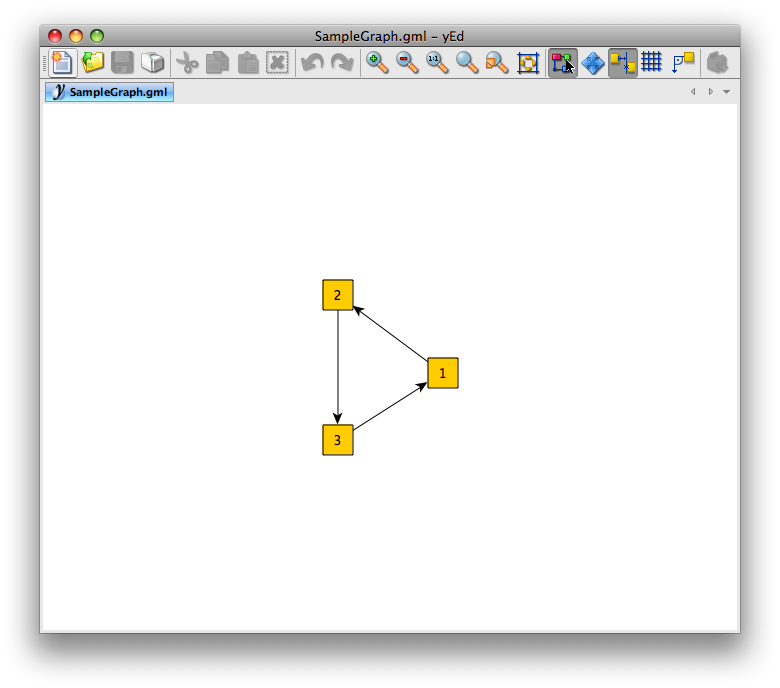
\includegraphics[scale=0.56]{pictures/SampleGraph.png}
\caption{Manual visualization of the sample graph}
\label{fig:sample_graph_yed_vis}
\end{figure}

Listing of the more complex graph with additional properties and is in the Appendix~A and the visualization of this graph shown in Figure~\ref{fig:yed_graph_vis}

\begin{figure}[h!]
\centering
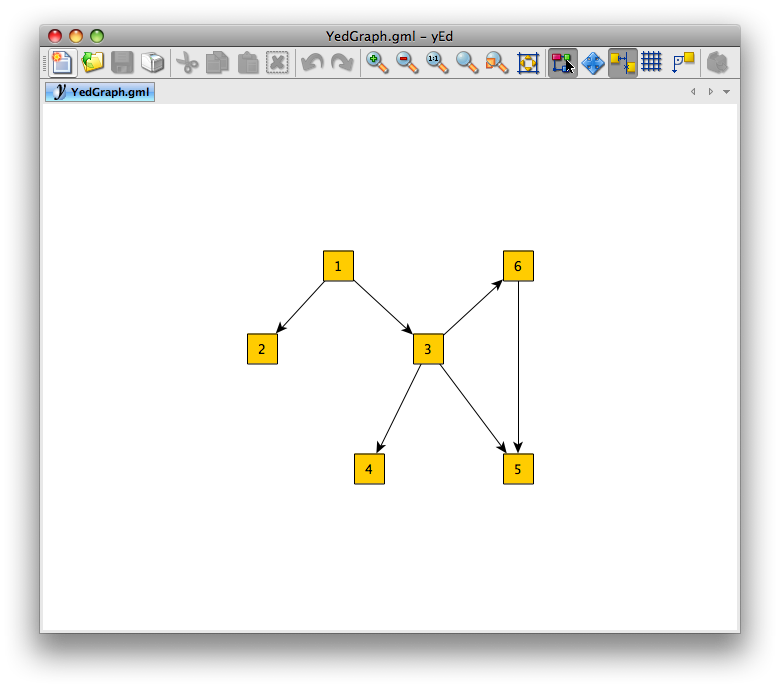
\includegraphics[scale=0.56]{pictures/YedGraph.png}
\caption{Manual visualization of the sample graph}
\label{fig:yed_graph_vis}
\end{figure}

Applications supporting GML~\cite{GML_wiki}

\begin{itemize}
\item Clairlib~\cite{clairlib}, a suite of open-source Perl modules intended to simplify a number of generic tasks in natural language processing (NLP), information retrieval (IR), and network analysis (NA).
\item Cytoscape~\cite{Cytoscape}, an open source bioinformatics software platform for visualizing molecular interaction networks, loads and save previously-constructed interaction networks in GML.
\item NetworkX~\cite{NetworkX}, an open source Python library for studying complex graphs.
\item ocamlgraph\cite{ocamlgraph}, a graph library for OCaml.
\item OGDF\cite{OGDF}, the Open Graph Drawing Framework, an open source C++ library containing implementations of various graph drawing algorithms. The library is self contained; optionally, additional packages like LP-solvers are required for some implementations.
\item Tulip~\cite{Tulip} (software) is a free software in the domain of information visualization capable of manipulating huge graphs (with more than 1.000.000 elements).
\item yEd~\cite{yed}, a free Java-based graph editor, supports import from and export to GML.
\end{itemize}

\subsection{Other Graph File Formats}

We choose to use GML because it is powerful enough for our needs and easy to implement. The next section covers several different graph file format we tried during the research. They are explained in descending order of interest.

\subsubsection{GraphML}
GraphML is a comprehensive and easy-to-use file format for graphs. It consists of a language core to describe the structural properties of a graph and a flexible extension mechanism to add application-specific data.~\cite{GraphML} Its main features include support of:
\begin{itemize}
\item directed, undirected, and mixed graphs;
\item hyper graphs;
\item hierarchical graphs;
\item graphical representations;
\item references to external data;
\item application-specific attribute data;
\item light-weight parsers;
\end{itemize}

The GraphML document consists of a graphml element and a variety of sub elements: graph, node, edge. Figure~\ref{fig:simple_graphml} below is a simple graph. It contains 11 nodes and 12 undirected edges.

\begin{figure}[h!]
\centering
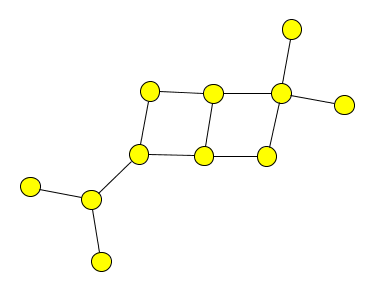
\includegraphics[scale=1.0]{pictures/simple.png}
\caption{A simple graph}
\label{fig:simple_graphml}
\end{figure}


And a corresponded graphml file is shown in Listing~\ref{simple_graphml_file}

\begin{center}
\renewcommand{\thelstlisting}{\thesection.\arabic{lstlisting}}
\begin{lstlisting} [language=xml, tabsize=1, caption={Simple graphml file}, captionpos=b, label=simple_graphml_file]
<graphml>
  <graph id="SampleGraph" edgedefault="undirected">
    <node id="node0"/>
    <node id="node1"/>
    <node id="node2"/>
    <node id="node3"/>
    <node id="node4"/>
    <node id="node5"/>
    <node id="node6"/>
    <node id="node7"/>
    <node id="node8"/>
    <node id="node9"/>
    <node id="node10"/>
    <edge source="node0" target="node2"/>
    <edge source="node1" target="node2"/>
    <edge source="node2" target="node3"/>
    <edge source="node3" target="node5"/>
    <edge source="node3" target="node4"/>
    <edge source="node4" target="node6"/>
    <edge source="node6" target="node5"/>
    <edge source="node5" target="node7"/>
    <edge source="node6" target="node8"/>
    <edge source="node8" target="node7"/>
    <edge source="node8" target="node9"/>
    <edge source="node8" target="node10"/>
  </graph>
</graphml>
\end{lstlisting}
\end{center}

GraphML support is implemented in the tool -- there is corresponded parsers to load graph from the GraphML file.

\subsubsection{DOT Graph File Format}
DOT is a plain text graph description language. It is a simple way of describing graphs in human readable form.

\begin{quotation}
``DOT graphs are typically files that end with the .gv (or .dot) extension.
At its simplest, DOT can be used to describe an undirected graph.
An undirected graph shows simple relations between objects, such as friendship between people.
The graph keyword is used to begin a new graph, and nodes are described within curly braces.
A double-hyphen (-\ -) is used to show relations between the nodes.''~\cite{DOT}
\end{quotation}

\begin{center}
\renewcommand{\thelstlisting}{\thesection.\arabic{lstlisting}}
\begin{lstlisting} [language=C, tabsize=1, caption={DOT file format: undirected graph}, captionpos=b]
graph graphname {
     a - - b - - c;
     b - - d;
}
\end{lstlisting}
\end{center}

Similar to undirected graphs, DOT can describe directed graphs, such as flowcharts and dependency trees.
The syntax is the same as for undirected graphs, except the digraph keyword is used to begin the graph, and an arrow ($->$) is used to show relationships between nodes.~\cite{DOT}

\begin{center}
\renewcommand{\thelstlisting}{\thesection.\arabic{lstlisting}}
\begin{lstlisting} [language=C, tabsize=1, caption={DOT file format: directed graph}, captionpos=b]
graph graphname {
     a -> b -> c;
     b -> d;
}
\end{lstlisting}
\end{center}

Visual representation of both graphs shown Figure~\ref{fig:dot_graphs} below.

\begin{figure}[h!]
\centering
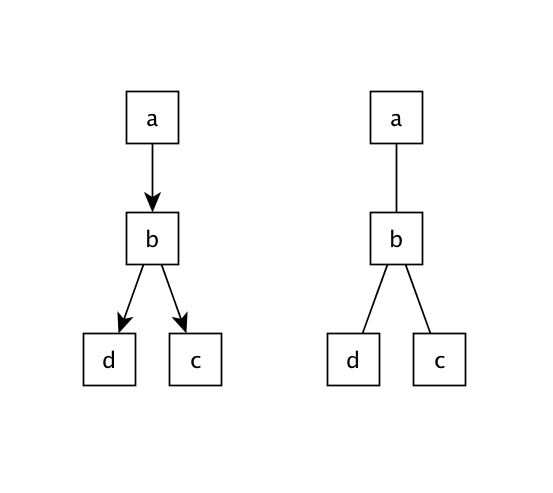
\includegraphics[scale=0.5]{pictures/dot_graph.png}
\caption{Directed and undirected graphs}
\label{fig:dot_graphs}
\end{figure}

\subsubsection{DGML}
DGML is an XML-based file format for directed graphs. Here is what a simple directed graph with three nodes and two links between them looks like

\begin{center}
\renewcommand{\thelstlisting}{\thesection.\arabic{lstlisting}}
\begin{lstlisting} [language=xml, tabsize=1, caption={DGML file format}, captionpos=b]
<?xml version="1.0" encoding="utf-8"?>
<directedGraph>
  <nodes>
    <node id="1" label="a" size="10"/>
    <node id="2" label="b" background="#FF008080"/>
    <node id="3" label="c" start="2010-06-10"/>
  </nodes>
  <links>
    <link source="1" target="2"/>
    <link source="2" target="3"/>
  </links>
  <properties>
    <property id="background" datatype="Brush"/>
    <property id="label" datatype="String"/>
    <property id="size" datatype="String"/>
    <property id="start" datatype="DateTime"/>
  </properties>
</directedGraph>
\end{lstlisting}
\end{center}

The complete XSD schema for DGML is available at Microsoft Schema web page~\cite{DGML_XSD_URL}.
DGML not only allows describing nodes and links in a graph,
but also annotating those nodes and links with any user defined property and/or category.

\subsubsection{GXL}
GXL (Graph eXchange Language) is an XML based exchange format for several kinds of graph information.
GXL provides a standardized notation for exchanging instance data (graph) including their structure (graph schema).

\begin{quotation}
``GXL was created to fulfill the need to exchange data between re-engineering tools.
Previously, interoperability between tools relied on converters between local formats.
This approach requires case-by-case negotiation of exchange semantics.
As the research area matured, it became apparent that a standard exchange format
was needed and that this format should provide a mechanism to help articulate semantics.''~\cite{GXL}.
\end{quotation}

GXL is considered as possible solution to transport graph data from different graph file formats

\subsubsection{SVG}
SVG is open graphical data storage format. Has been in development since 1999 by a group of companies within the W3C. SVG drew on experience from the designs of two older formats: Precision Graphics Markup Language (PGML) developed from Adobe's PostScript and Vector Markup Language (VML) developed from Microsoft's RTF. Which were submitted to W3C in 1998.


SVG allows three types of graphic objects:
\begin{itemize}
\item Vector graphics
\item Raster graphics
\item Text
\end{itemize}

\begin{quotation}
``Graphical objects, including PNG and JPEG raster images, can be grouped, styled, transformed,
and composited into previously rendered objects. SVG does not directly support z-indices
that separate drawing order from document order for overlapping objects, unlike some other vector mark up languages like VML.
Text can be in any XML name space suitable to the application, which enhances search ability and accessibility of the SVG graphics.
The feature set includes nested transformations, clipping paths, alpha masks, filter effects, template objects and extensibility..''~\cite{SVG}
\end{quotation}

As described above current information storage format is not meant to store graphs but is considered as possible data exchange storage format for the export functionality -- export graph visualization in the file to view it in any modern browser.

\subsection{OpenGL Visualization Standard}
\label{sec:opengl}
During first attempts to visualize data using available libraries the performance became a bottleneck. Without any measurement methods it was obvious that Java3D API used in the most of the libraries does not allow smooth intersections and real-time computations.


As possible solutions we introduces our own abstraction for visualization using OpenGL and underlying hardware acceleration.


OpenGL is a software interface to graphics hardware. This interface consists of about 120 distinct commands,
which you use to specify the objects and operations needed to produce interactive three-dimensional applications.
OpenGL is designed to work efficiently even if the computer that displays the graphics you create is not the computer that runs your graphics program.

\begin{quotation}
``OpenGL is designed as a streamlined, hardware-independent interface to be implemented on many different hardware platforms.
To achieve these qualities, no commands for performing windowing tasks or obtaining user input are included in OpenGL;
instead, you must work through whatever windowing system controls the particular hardware you're using.
Similarly, OpenGL doesn't provide high-level commands for describing models of three-dimensional objects.
Such commands might allow you to specify relatively complicated shapes such as automobiles, parts of the body, airplanes,
or molecules. With OpenGL, you must build up your desired model from a small set of geometric primitive --- points,
lines, and polygons.''~\cite{THE_RED_BOOK}
\end{quotation}

Since OpenGL is not bound to actual hardware but it is implemented as native C library and coupled to the Operation System it is run on. To avoid direct calls from the Java program to native API (Java Native Interface) we used wrapper.

There are many wrappers over OpenGL for developing on different programming languages.
One of the favorite in the Java community are JOGL and LWJGL.

\begin{quotation}
``The Lightweight Java Game Library (LWJGL) is a solution aimed directly at professional and amateur Java programmers
alike to enable commercial quality games to be written in Java. LWJGL provides developers access to
high performance cross platform libraries such as OpenGL and OpenAL (Open Audio Library) allowing for state of the art
3D games and 3D sound. Additionally LWJGL provides access to controllers such as Gamepads, Steering wheel and Joysticks.
All in a simple and straight forward API.
LWJGL is available under a BSD license, which means it is open source and freely available at no charge.''~\cite{LWJGL}
\end{quotation}


In the thesis used JOGL wrapper library over OpenGL. Java OpenGL (JOGL) is a wrapper library that allows OpenGL to be used in more Java way. Here is the overview of the JOGL project:

\begin{quotation}
``The base OpenGL C API and associated operation system API, are accessed in JOGL via Java Native Interface (JNI) calls.
As such, the underlying system must support OpenGL for JOGL to work.
JOGL differs from some other Java OpenGL wrapper libraries in that it merely exposes the procedural OpenGL API
via methods on a few classes, rather than trying to map OpenGL functionality onto the object-oriented programming paradigm.
Indeed, most of the JOGL code is auto generated from the OpenGL C header files via a conversion tool named GlueGen,
which was programmed specifically to facilitate the creation of JOGL.

This design decision has both its advantages and disadvantages.
The procedural and state machine nature of OpenGL is inconsistent with the typical method of programming under Java,
which is bothersome to many programmers. However, the straightforward mapping of the OpenGL C API to Java methods
makes conversion of existing C applications and example code much simpler.
The thin layer of abstraction provided by JOGL makes runtime execution quite efficient,
but accordingly is more difficult to code compared to higher-level abstraction libraries like Java3D.
Because most of the code is auto generated.''~\cite{JOGL}
\end{quotation}


\subsection{Program Architecture}

An overview on the tool's architecture is given in Figure~\ref{fig:modules}. The implementation is divided into several modules specialized for various tasks.
The \textsf{IO} module implements data loading from gml files. The data is stored in extended gml file format,
which contains additional properties for nodes, such as the node label.
The \textsf{Graph Core} module extends the JUNG graph model~\cite{JUNG} in order to fit it to our requirements.
The implementation of Swing GUI and OpenGL user interactions is realized by the \textsf{User Interaction} module.
The \textsf{Graph Visualization} module and its submodules contain all code for the whole visualization process,
including our own layout implementation, primitive drawing abstraction, and program state machine.
One of the most important modules of \tool\ is of course \textsf{Subgraph Extraction} that contains the implementation of the subtree calculation algorithm.

\begin{figure}[h!]
\centering
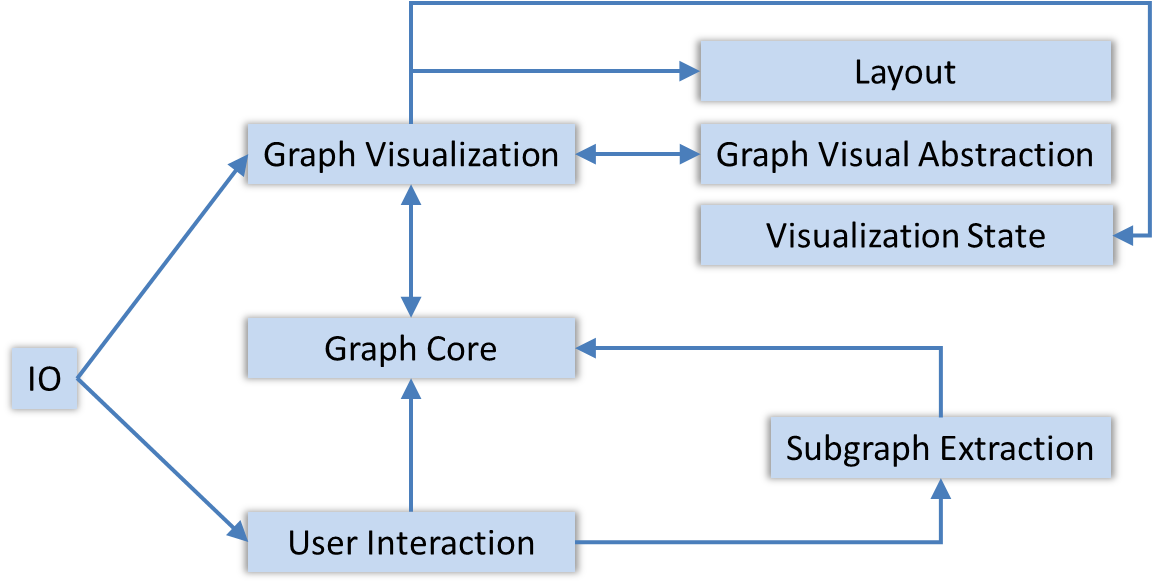
\includegraphics[scale=0.62]{pictures/modules.png}
\caption{Module architecture of GoClusterViz tool}
\label{fig:modules}
\end{figure}

One of the main module in the program is \textsf{Subgraph Extraction} module. Extraction algorithm was explained in Section~\ref{sec:algorithm} and in the Appendix~A is pseudo-code, implementation is in the class \textsf{se.lnu.thesis.algorithm.Extractor}.

Complete UML class diagram of the GoClusterViz can be found in the Appendix~C. Here is a brief overview of the package content.

Main class and program entry point is class --- \textsf{GoClusterViz}.

Package \textsf{se.lnu.thesis.gui} contains all interface abstractions and Swing implementations for main window, menus and event handling.

\textsf{se.lnu.thesis.element} is hierarchy for graph visualization. It is implementation of the Composite pattern:

\begin{quotation}
``In software engineering, the composite pattern is a partitioning design pattern.
The composite pattern describes that a group of objects are to be treated in the same way as a single instance of an object.
The intent of a composite is to `compose' objects into tree structures to represent part-whole hierarchies.
Implementing the composite pattern lets clients treat individual objects and compositions uniformly.''~\cite{COMPOSITE_GAMMA}
\end{quotation}

\begin{figure}[h!]
\centering
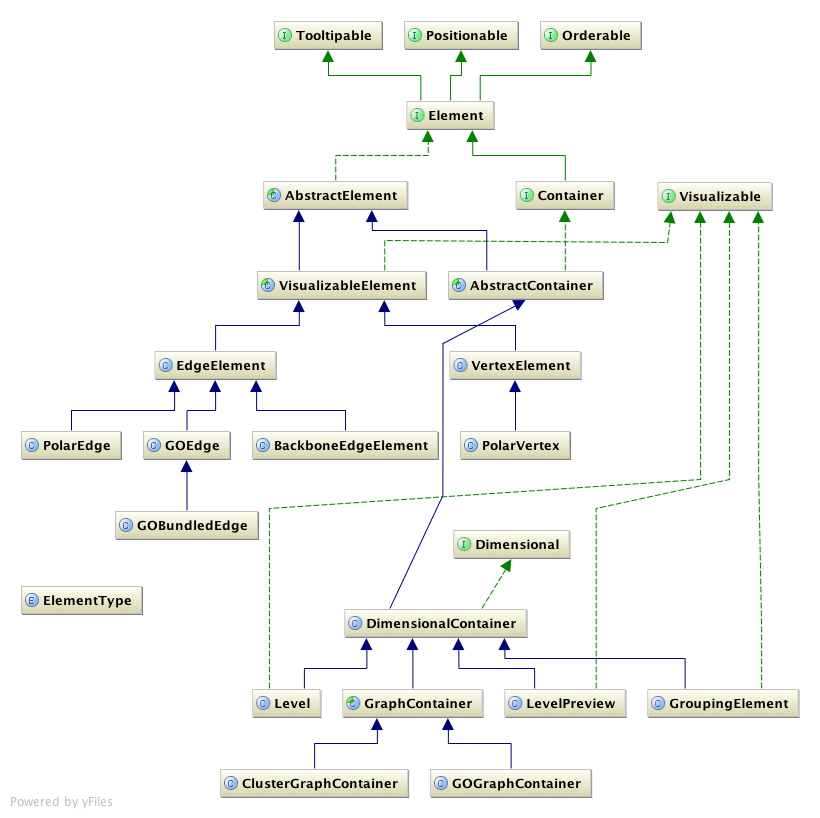
\includegraphics[scale=0.42]{pictures/uml_elements.png}
\caption{Graph elements visualisation hierarchy abstraction}
\label{fig:uml_elements}
\end{figure}

Package \textsf{se.lnu.thesis.paint} contains all drawing implementations.
Graph elements do not implement visualization shape, for that purpose there is \textsf{ElementVisualizer} abstraction. Diagram in Figure~\ref{fig:uml_visualizers} shows complete UML diagram of the package \textsf{se.lnu.thesis.paint.visualizer}, there are several different shape visualizer. To reduce memory usage all visualizers are stored in the \textsf{ElementVisualizerFactory} --- Flyweight design pattern.

\begin{quotation}
``Flyweight is a software design pattern.
A flyweight is an object that minimizes memory use by sharing as much data as possible with other similar objects;
it is a way to use objects in large numbers when a simple repeated representation would use an unacceptable amount of memory.
The term is named after the boxing weight class.
Often some parts of the object state can be shared and it is common to put them in external data structures and pass them to
the flyweight objects temporarily when they are used.''~\cite{FLYWEIGHT}
\end{quotation}

Flyweight pattern is used to store different kind of visualizers for graph elements. It means for each element of the graph there is a reference to visualizer object containing its shape, metrics, and other formatting data, which reduce amount of data to hundreds or thousands of bytes for each character. For every element of the graph there is a reference to a flyweight visualizer object shared by every instance of the same graph element in the graph; only the position of each element and current state (selected, highlighted, focused) is stored internally.

\begin{figure}[h!]
\centering
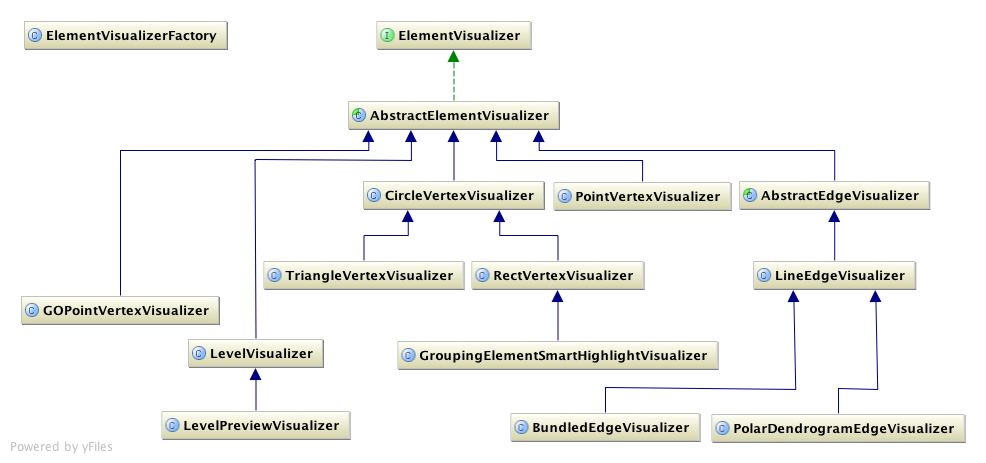
\includegraphics[scale=0.41]{pictures/uml_visualizers.png}
\caption{Flyweight element visualizers}
\label{fig:uml_visualizers}
\end{figure}

User interaction state machine is implementation of the State software development pattern located in the package \textsf{se.lnu.thesis.paint.state}.

\begin{quotation}
``A monolithic objects behavior is a function of its state, and it must change its behavior at run-time depending on that state.
Or, an application is characterized by large and numerous case statements that vector flow of control based on the state
of the application. The State pattern does not specify where the state transitions will be defined. The choices are two:
the context object, or each individual State derived class.
The advantage of the latter option is ease of adding new State derived classes.
The disadvantage is each State derived class has knowledge of (coupling to) its siblings,
which introduces dependencies between subclasses.
A table-driven approach to designing finite state machines does a good job of specifying state transitions,
but it is difficult to add actions to accompany the state transitions. The pattern-based approach uses code
(instead of data structures) to specify state transitions,
but it does a good job of accommodating state transition actions.''~\cite{STATE}
\end{quotation}

It means that graph has several states: normal view, zoomed view, lens is on the scene, etc.
It releases the code from the long ``switch'' statements  and determines logic into different classes.

\begin{figure}[h!]
\centering
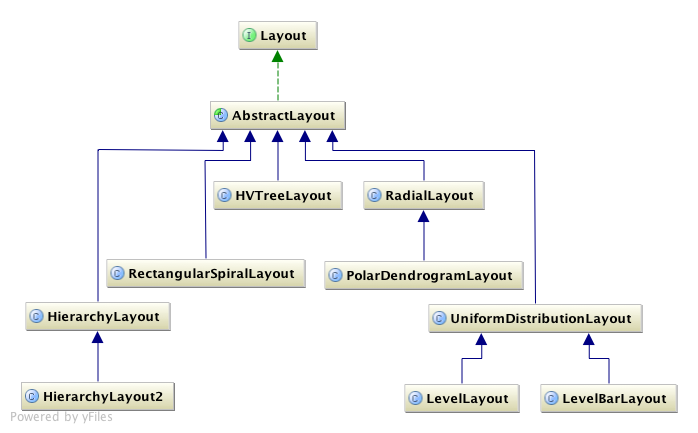
\includegraphics[scale=0.55]{pictures/uml_layouts.png}
\caption{Layouts class diagram}
\label{fig:uml_layouts}
\end{figure}


During this work several layouts were implemented, as it was discussed earlier.
Layout implementations are in the \textsf{se.lnu.thesis.layout} package. UML class diagram is shown on Figure~\ref{fig:uml_layouts}.

\newpage
\section{Conclusion and Future Work}
\label{sec:conclusion}

We presented a new method for the combined visualization of an ontology (represented as DAG)
and an hierarchical clustering (represented as tree) of one data set.
The proposed method interactively visualizes all the data without scrolling,
thereby presenting an complete overview.
It also allows for interactive selection and navigation to explore the data.
The provided visualization approach and the implementation have shown that the program is able to tackle the problem in our research focus ---
the visualization and visual mapping between two huge and conceptually different data sets.

However, there are some improvements that should be performed in the future.

As explained previously in the Section~\ref{sec:go}, the zoomed-in view for the GO shows three levels at the same time while displaying the subgraph by highlighting the nodes only.
The edges are omitted due to clutter problems that can occur since edges from a higher level might go through the zoomed-in view to nodes in the lower layers.
Since we are zoomed in, this does no make sense to show, because we have no insight from which layer those edges are coming from, nor to which layer they are going to.
However, an improvement is possible by showing only edges between the three layers shown in the zoomed-in GO view.
At the same time, the edge bundling algorithm could also be improved.

The thesis application is not a general visualization tool.
It has been developed especially for the biology scientists and is driven by their requirements which means that the application fulfills their needs.
There is no application with the same functionality.
Visualization technique developed during the work is based on provided data, uses its specific structure as advance.
On the other hand the visualization approach may apply to another fields.

As for a future improved version of the rectangular spiral metaphor, is to draw smaller similar spirals instead of aggregating sub-trees into rectangles.
For smaller sub-trees this approach will help to see the structure without lens.

For better user experience, it is possible to provide an animation for different events:
lens appearing and hiding in the cluster graph,
smooth level scrolling in the Gene Ontology visualization,
step-by-step elements highlighting.

\newpage
\addcontentsline{toc}{section}{References}

\begin{thebibliography}{99}

\mywebref{VLSI}{VLSI}{http://en.wikipedia.org/wiki/Very-large-scale_integration}
\mywebref{Graph_drawing}{Graph drawing general information}{http://en.wikipedia.org/wiki/Graph_drawing}

\bibitem{Radial_dendrogram}
P. Imrich, K. Mueller, D. Imre, A. Zelenyuk, And W. Zhu, Interactive Poster: A Hardware-Accelerated Rubbersheet Focus + Context Technique For Radial Dendrograms, IEEE Information Visualization Symposium '03 Seattle, October 2003

\mywebref{Dendrogram}{Introduction into Dengrograms}{en.wikipedia.org/wiki/Dendrogram}

\bibitem{Barlow_Neville}
T. Barlow and P. Neville, A comparison of 2D visualization of hierarchies, Information Visualization pp 131-138, 2001.

\bibitem{Kreussler_Schumann}
M. Kreussler and H. Schumann, A flexible approach for visual data mining, IEEE Trans. VisualGraphics, vol. 8, no. 1, pp. 39-51, 2002.

\bibitem{Yang_Ward}
J. Yang, M. Ward, and E. Rundensteiner, InterRing: An interactive tool for visually navigating and manipulating hierarchical structures, IEEE 2002 Symposium on Information Visualization, pp. 77-92, 2002.


\mywebref{Biology}{Biotech}{http://biotech.icmb.utexas.edu/pages/bioinfo.html}

\mywebref{Bioinformatic}{Bioinformatic definition information is}{http://www.absoluteastronomy.com/topics/Bioinformatics}

\mywebref{Bioinformatic_resources}{Bioinformatic resources page}{http://www.bibalex.org/cssp/Event/Attachments/Bioinformatics resources.pdf}

\mywebref{GO_website}{Gene Ontology project homepage}{http://www.geneontology.org/}

\mywebref{OBO}{The Open Biomedical Ontologies}{http://www.obofoundry.org/}

\bibitem{data_clustering_book}
G. Gan, C. Ma and J. Wu, Data Clustering. Theory, Algorithms, and Applications, Society for Industrial and Applied Mathematics pp 3, 2007.

\mywebref{Kerren}{Prof. Dr. Andreas Kerren home page}{http://homepage.lnu.se/staff/akemsi/}
\mywebref{Schreiber}{Prof. Dr. Falk Schreiber home page}{http://bic-gh.ipk-gatersleben.de/~schreibe/}
\mywebref{ISOVIS}{ISOVIS research group home page}{http://cs.lnu.se/isovis/}
\mywebref{PBG}{Plant Bioinformatic research Group home page}{http://nwg.bic-gh.de/}

\mywebref{Graphlet}{Graphlet project homepage}{http://www.fmi.uni-passau.de/Graphlet/}
\mywebref{GML}{GML file format explanation}{http://www.infosun.fim.uni-passau.de/Graphlet/GML/gml-tr.html}
\mywebref{GML_wiki}{GML supported programs}{http://en.wikipedia.org/wiki/Graph_Modelling_Language}
\mywebref{yed}{yEd project homepage}{http://www.yworks.com/en/products_yed_about.html}
\mywebref{clairlib}{Clairlib}{http://www.clairlib.org/}
\mywebref{Cytoscape}{Cytoscape}{http://en.wikipedia.org/wiki/Cytoscape}
\mywebref{NetworkX}{NetworkX}{http://en.wikipedia.org/wiki/NetworkX}
\mywebref{ocamlgraph}{ocamlgraph}{http://ocamlgraph.lri.fr/}
\mywebref{OGDF}{OGDF}{http://www.ogdf.net/}
\mywebref{Tulip}{Tulip}{http://tulip.labri.fr/TulipDrupal/}
\mywebref{GraphML}{GraphML specification}{http://graphml.graphdrawing.org/}
\mywebref{DOT}{DOT graph language}{http://en.wikipedia.org/wiki/DOT_language}
\mywebref{DGML_XSD_URL}{DGML XSD schema}{http://schemas.microsoft.com/vs/2009/dgml/}
\mywebref{GXL}{GXL introduction}{http://www.gupro.de/GXL/Introduction/section1.html}
\mywebref{SVG}{SVG information}{http://en.wikipedia.org/wiki/Scalable_Vector_Graphics}
\mywebref{GDC}{Graph Drawing Conference '95}{www.informatik.uni-trier.de/~ley/db/conf/gd/gd95.html}

\bibitem{EDGE_BUNDLING_1}
Danny Holten, Hierarchical Edge Bundles: Visualization of Adjacency Relations in Hierarchical Data, IEEE Transactions On Visualization and Computer Graphics 2006, Volume 12, Number 5

\bibitem{EDGE_BUNDLING_2}
Danny Holten, Jarke J. van Wijk, Force-Directed Edge Bundling for Graph Visualization, Eurographics/ IEEE-VGTC Symposium on Visualization 2009, Volume 28 (2009), Number 3

\mywebref{java_com}{Java FAQ}{http://www.java.com/en/download/faq/whatis_java.xml}

\mywebref{BINARY_TREE}{Binary Tree definition}{http://www.wordiq.com/definition/Binary_tree}

\mywebref{JAVA_2D}{Java 2D reference}{http://java.sun.com/products/java-media/2D/reference/index.html}

\mywebref{JAVA_AWT}{Java AWT overview}{http://en.wikipedia.org/wiki/Abstract_Window_Toolkit}

\mywebref{JAVA_SWING}{Java SWING overview}{http://en.wikipedia.org/wiki/Swing_(Java)}

\mywebref{AWT_VS_SWING}{AWT vs SWING comparison}{http://edn.embarcadero.com/article/26970}

\mywebref{MAVEN_HOME_PAGE}{Maven project home page}{http://maven.apache.org/}

\mywebref{APACHE_FOUNDATION_HOME_PAGE}{Apache Foundation home page}{http://www.apache.org/}

\bibitem{MAVEN_BOOK_1}
Vincent Massol, Jason van Zyl, Better builds with Maven, Mergere Library Press, pp. 16, 2006.

\bibitem{MAVEN_BOOK_2}
Vincent Massol, Jason van Zyl, Better builds with Maven, Mergere Library Press, pp. 18, 2006.

\mywebref{REVISION_CONTROL}{Revision Control definition}{http://en.wikipedia.org/wiki/Revision_control}

\mywebref{GIT}{Git overview}{http://en.wikipedia.org/wiki/Git_(software)}

\mywebref{GitHub_homepage}{Project home page on GitHub}{http://github.com/vadyalex/thesis}

\mywebref{GitHub_repository}{Project Git repository}{git://github.com/vadyalex/thesis.git}

\mywebref{GEF}{Java Graph Editing Framework}{http://gef.tigris.org/}

\mywebref{ILOG_Jview}{ILOG Jview}{http://www.ilog.com/products/jviews/}

\mywebref{JGraphT}{JGraphT)}{http://jgrapht.sourceforge.net/}

\mywebref{JUNG}{Java Universal Network / Graph Framework (JUNG)}{http://jung.sourceforge.net/}

\mywebref{JUNG_OVERVIEW}{JUNG graph library overview}{http://jung.sourceforge.net/index.html}

\mywebref{EXTC}{ExtC}{http://code.google.com/p/ext-c/}

\mywebref{DJINN}{Djinn}{http://www.jnovation.net/djinn}

\mywebref{ANGUR}{Angur}{http://angur.sourceforge.net/}

\mywebref{RDF_GRAVITY}{RDF Gravity}{http://semweb.salzburgresearch.at/apps/rdf-gravity/index.html}

\mywebref{GUESS}{GUESS}{http://www.hpl.hp.com/research/idl/projects/graphs/index.html}

\mywebref{ADAPTNET}{ADAPTNet}{http://bioinformatics.picr.man.ac.uk/adaptnet}

\bibitem{AUGUR}
Cleidson de Souza, Jon Froehlich, Paul Dourish, Seeking the Source: Software Source Code as a Social and Technical Artifact, GROUP '05 Proceedings of the 2005 international ACM SIGGROUP conference on Supporting group work

\mywebref{AUGUR_2}{Jon Froehlich web page}{http://www.cs.washington.edu/homes/jfroehli/}

\mywebref{ARIADNE}{Ariadne project homepage}{http://awareness.ics.uci.edu/~ariadne/}

\mywebref{NETSIGHT}{Netsight}{http://jung.sourceforge.net/netsight}

\mywebref{INFOVIS_CYBERINFRASTRUCTURE} {InfoVis CuberInfrastructure}{http://iv.slis.indiana.edu/sw/}

\mywebref{PWCOMP}{PWComp project homepage}{http://www.ocf.berkeley.edu/~jadelman/pwcomp/index.html}

\mywebref{GOOGLE_CARTOGRAPHY}{Google Cartography}{http://richard.jones.name/google-hacks/google-cartography/google-cartography.html}

\mywebref{GINY}{GINY}{http://csbi.sourceforge.net/}

\mywebref{GRAPHEXPLORER}{GraphExplorer}{http://graphexplore.cgt.duke.edu/}

\mywebref{TOTEM}{TOTEM}{http://totem.run.montefiore.ulg.ac.be/}

\mywebref{D2K}{D2K}{http://alg.ncsa.uiuc.edu/do/downloads}

\mywebref{GRAPHBUILDER}{graphBuilder project homepage}{http://data.aad.gov.au/analysis/gb.cfm}

\mywebref{SEMIOPHORE}{Semiophore}{http://www.semiophore.net/}

\mywebref{XHOLON}{Xholon}{http://sourceforge.net/projects/xholon/}

\mywebref{FLINK}{Flink}{http://flink.semanticweb.org/}

\mywebref{SWC}{Semantic Web Challenge introduction}{http://challenge.semanticweb.org/}

\mywebref{T_PROX}{T-Prox}{http://www.t-prox.net/}

\mywebref{SIMPLE_C_K_EDITOR}{Simple C-K Editor introduction}{http://code.google.com/p/ckeditor}

\mywebref{PCOPGENE}{PCOPGene}{http://revolutionresearch.uab.es/}

\bibitem{THE_RED_BOOK}
Dave Shreiner, Mason Woo, Jackie Neider, Tom Davis, OpenGL(R) Programming Guide: The Official Guide to Learning OpenGL(R), Version 2.1 (6th Edition), Addison-Wesley Professional, 2007.

\mywebref{LWJGL}{LWJGL}{http://www.lwjgl.org/}

\mywebref{JOGL}{JOGL}{http://jogamp.org/}

\mywebref{Piccolo}{Piccolo}{http://www.cs.umd.edu/hcil/jazz/}

\mywebref{VTK}{Visualisation Toolkit}{http://www.vtk.org/}

\mywebref{InfoVis_Toolkit}{InfoVis Toolkit}{http://ivtk.sourceforge.net/}

\mywebref{Improvise}{Improvise project homepage}{http://www.cs.ou.edu/~weaver/improvise/index.html}

\bibitem{COMPOSITE_GAMMA}
Erich Gamma, Richard Helm, Ralph Johnson, John M. Vlissides, Design Patterns: Elements of Reusable Object-Oriented Software. Addison-Wesley., 1995, pp. 395.

\mywebref{FLYWEIGHT}{Flyweight design pattern explanation}{http://en.wikipedia.org/wiki/Flyweight_pattern}

\mywebref{STATE}{State design pattern explanation}{http://sourcemaking.com/design_patterns/state}

\end{thebibliography}

\setcounter{section}{0}

\newpage
\myappendix{Listing of a Complex GML File}
\label{sec:appendix_A}

\begin{center}
	\lstinputlisting[language=xml, tabsize=2, basicstyle=\footnotesize, numberstyle=\footnotesizefr]{graphs/YedGraph.gml}
\end{center}

\newpage
\section*{Appendix B: Subgraph extraction algorithm}
\addcontentsline{toc}{section}{Appendix B: Subgraph extraction algorithm}
\label{sec:appendix_B}

\begin{center}
\small
\begin{lstlisting}[language=Java]
// selected vertex in the Gene Ontology by user
GO_vertex;

if GO_vertex is in cache {
  // already computed, load from cache
  load from cache GO_subgraph and Cluster_subgraph;
  return;
}

// extract subgraph using non-recursive DFS
// starting from vertex GO_vertex as root
GO_subgraph = extractSubgraph(GO_graph, GO_vertex);
save GO_subgraph to cache with key GO_vertex

// create empty subgraph
Cluster_subtree = new Graph;

for each vertex in GO_subgraph {
  if vertex is leaf {
    // leaf labels are the same for both graphs,
    // but vertex objects are different
    l_label = GO_graph.getLabel(vertex);
    leaf = Cluster_graph.getVertexByLabel(l_label);
    // get all connected vertices
    // from current leaf up to the Cluster root
    connectedVertices = invertDFS(Cluster_graph, leaf);

    // add connected vertices to cluster subtree
    // create edges
    for (int i=0; i<=connectedVertices.size()-1; i++) {
      node1, node2 = null;
      node1 = connectedNodes.get(i);
      Cluster_subtree.addVertex(node1);

      if (i+1<=connectedNodes.size()-1) {
      node2 = connectedNodes.get(i+1);

      Cluster_subtree.addVertex(node2);
      Cluster_subtree.addEdge(node2,node1);
    }
  }

  // find lowest common root for subgraph
  // and remove vertices from the root to common root
  removeRootChain(Cluster_graph, Cluster_subtree);
}

save Cluster_subtree to cache with key GO_vertex
\end{lstlisting}
\end{center}

\newpage
\myappendix{Complete UML Class Diagram}
%\addcontentsline{toc}{section}{Appendix C: Complete UML Class Diagram}
\label{sec:appendix_C}

\begin{figure}[h!]
\centering
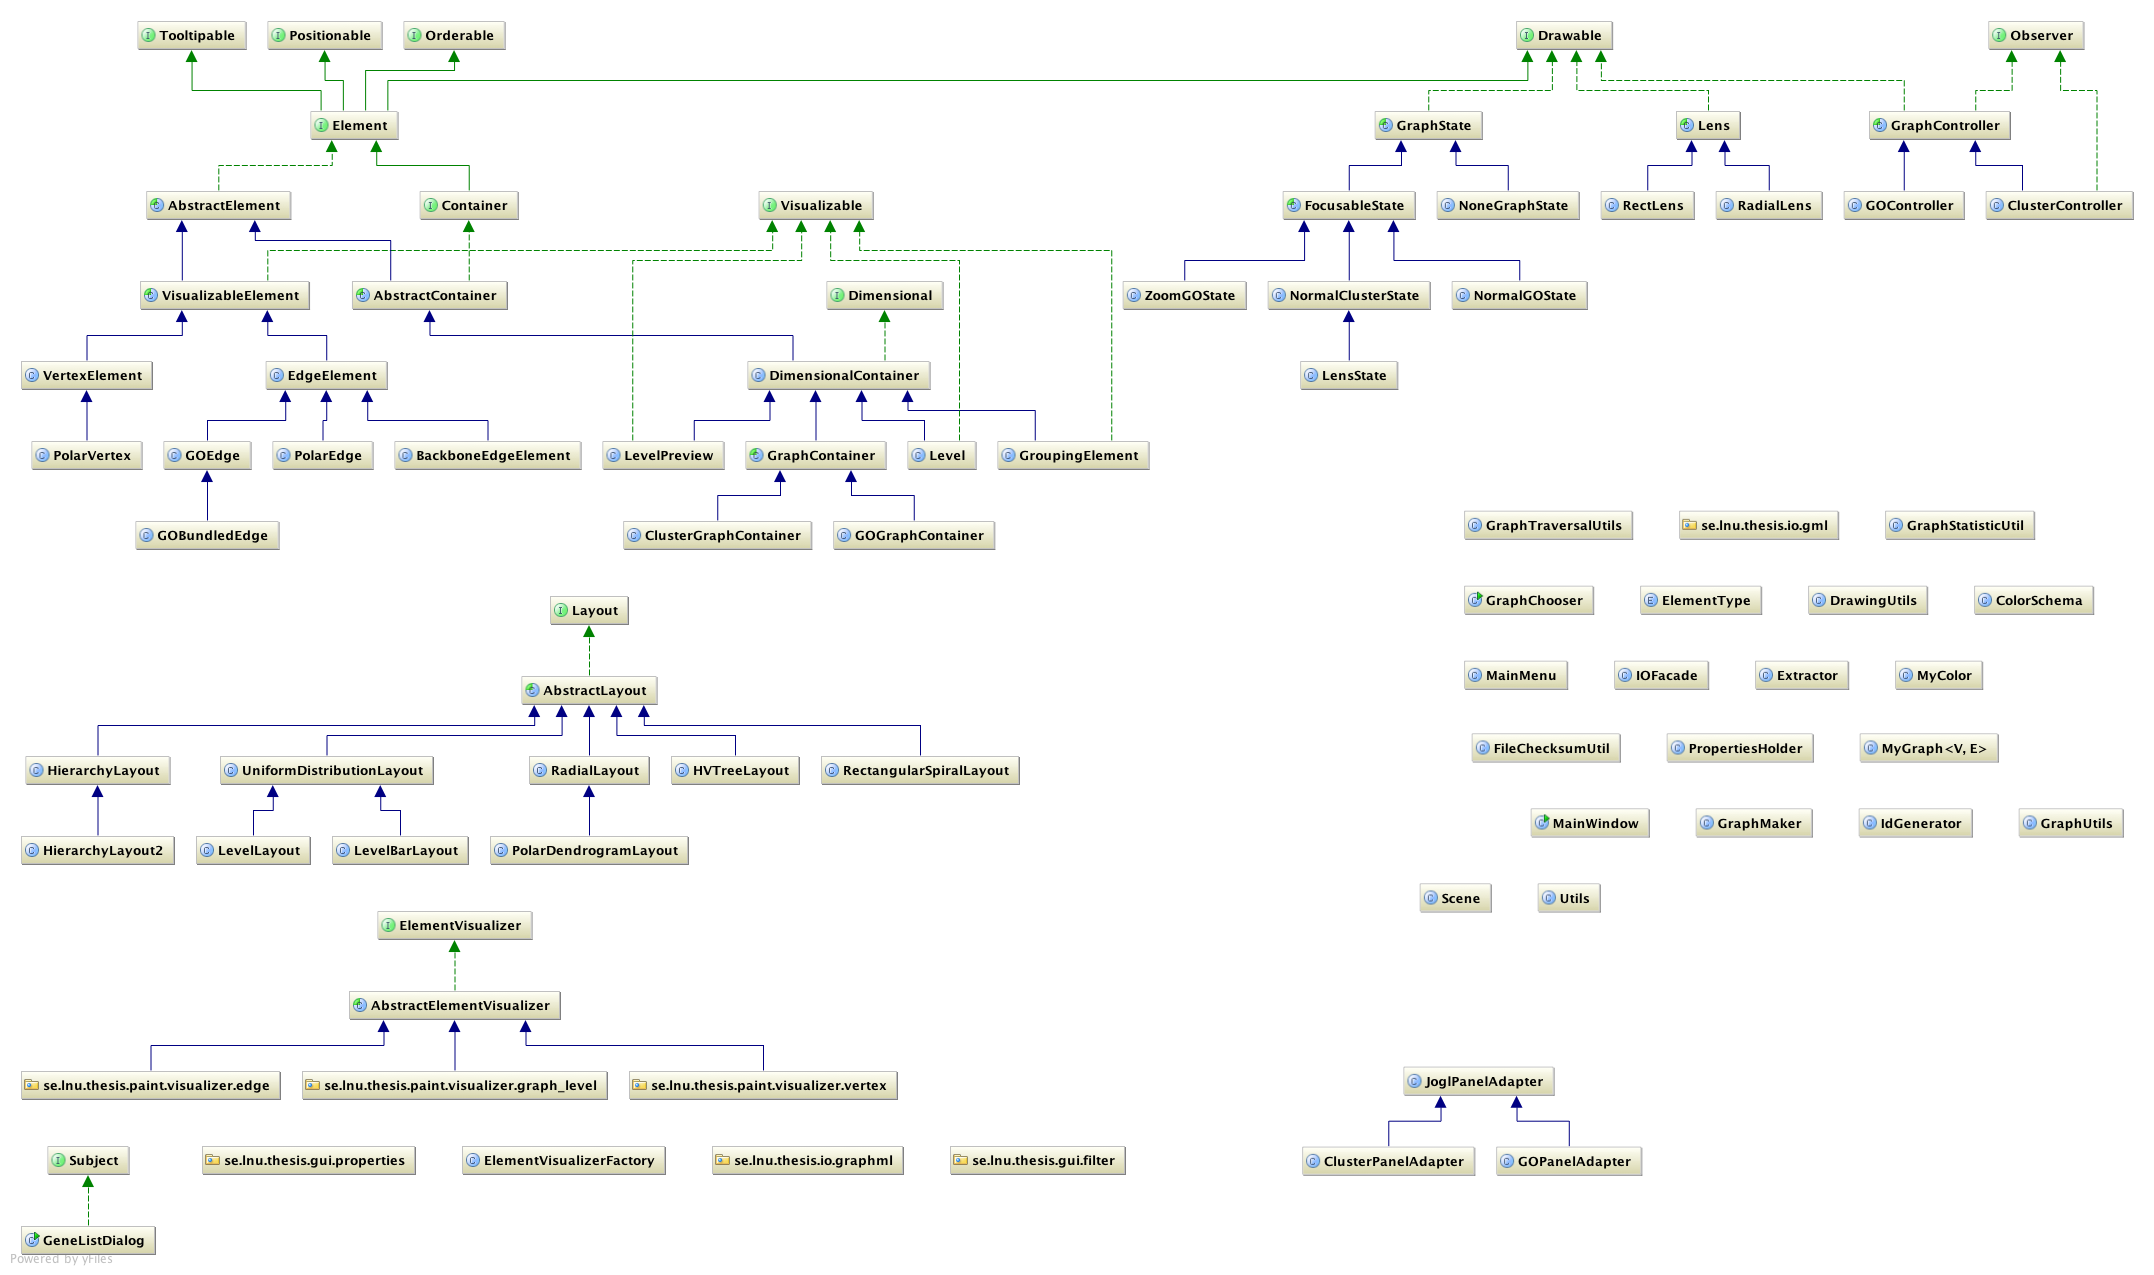
\includegraphics[scale=0.31, angle=90]{pictures/uml_diagram.png}
\end{figure}

\newpage
\myappendix{Program Execution Screenshots}
%\addcontentsline{toc}{section}{Appendix D: Program Execution Screenshots}
\label{sec:appendix_D}

\begin{figure}[h!]
\centering
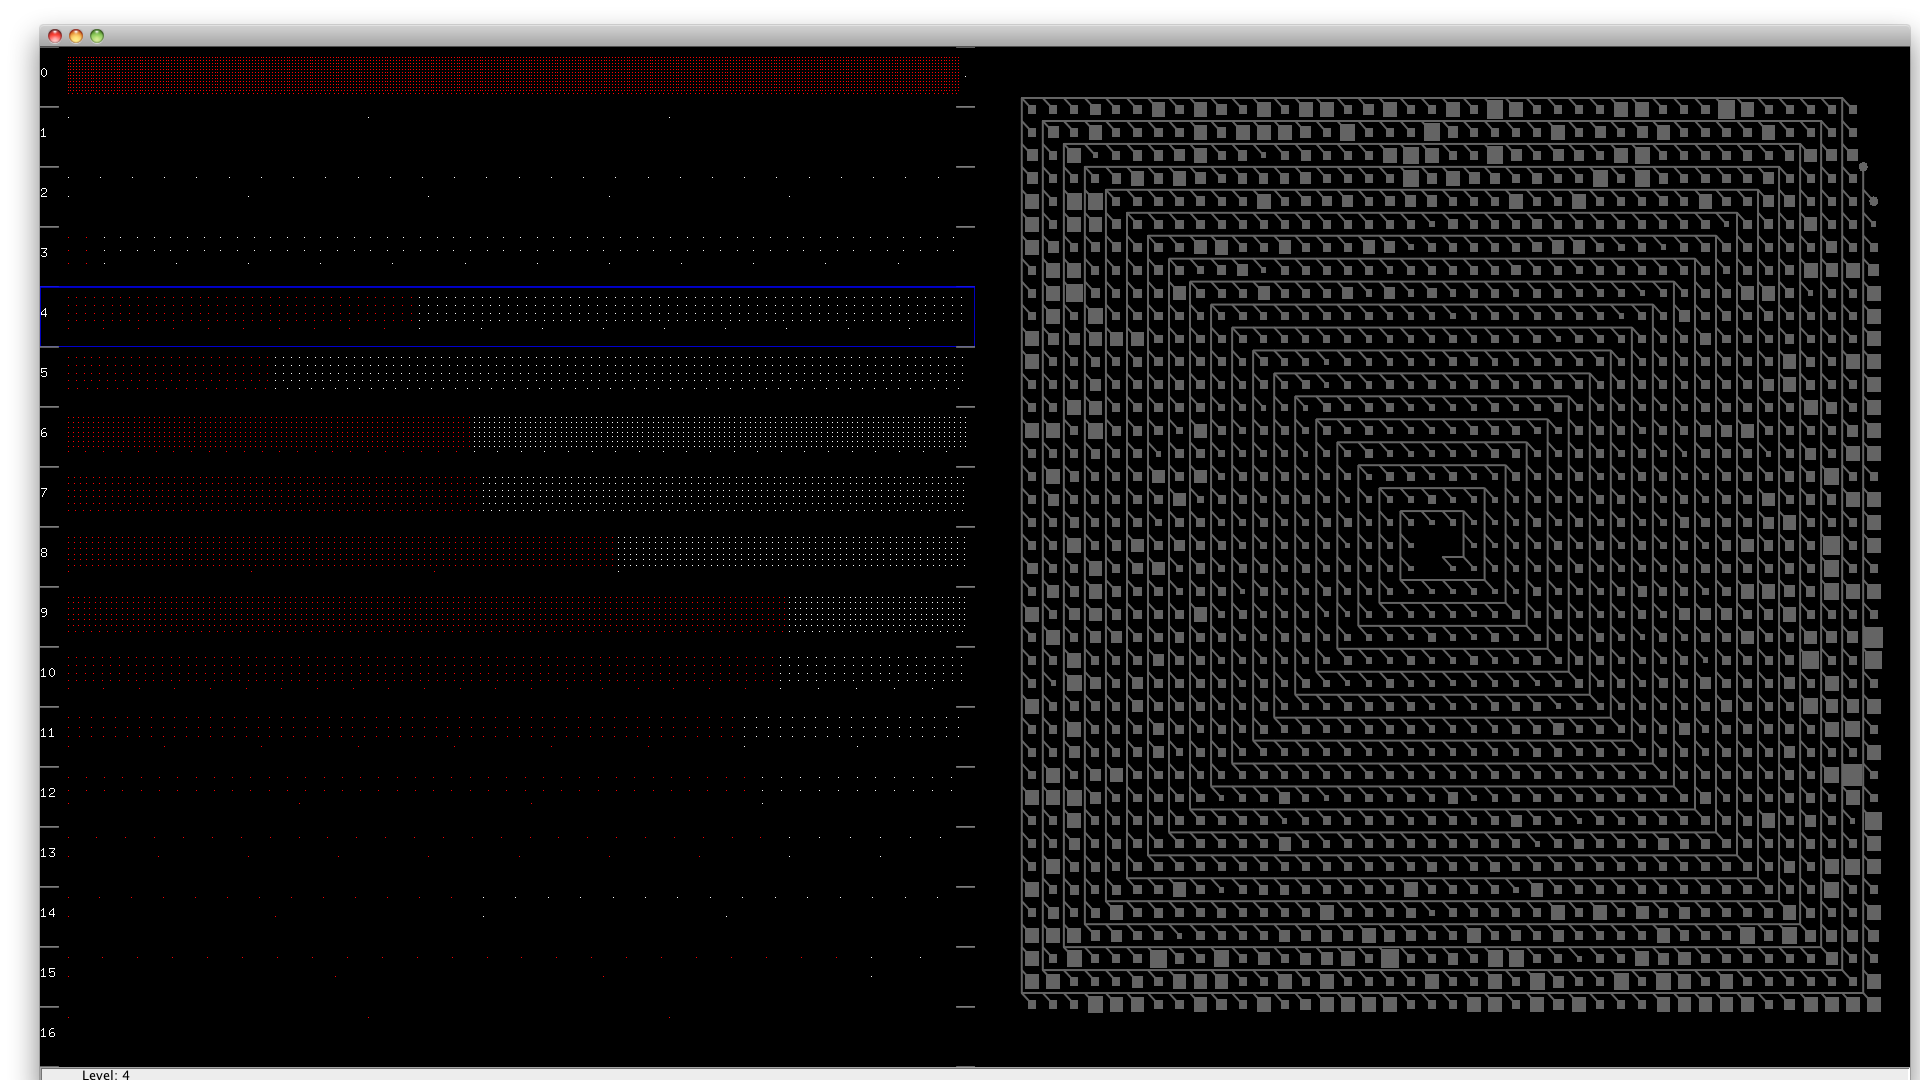
\includegraphics[scale=0.33, angle=90]{pictures/screenshot_1.png}
\caption{Visualization of the Gene Ontology graph by levels and Cluster analysis result graph. Blue rectangle -- highlighted level 4}
\end{figure}

\newpage
\begin{figure}[h!]
\centering
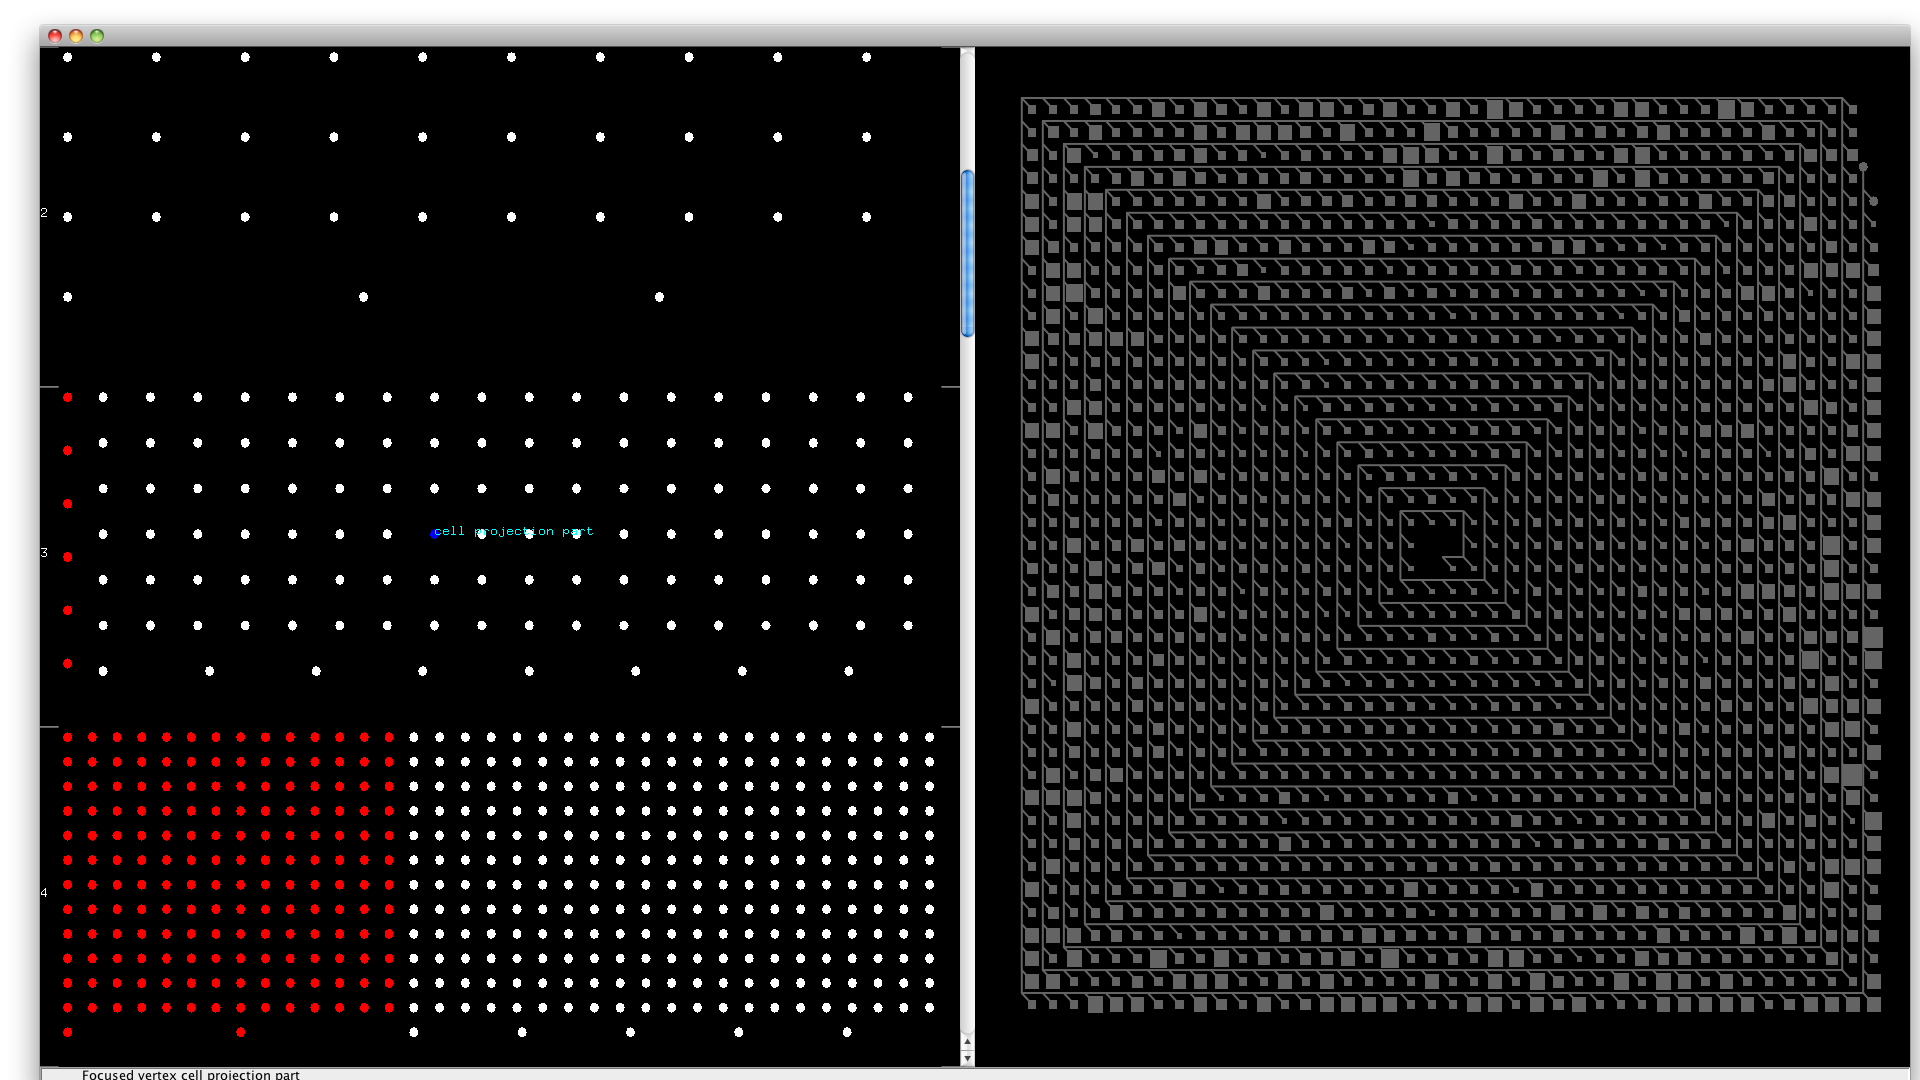
\includegraphics[scale=0.33, angle=90]{pictures/screenshot_2.png}
\caption{Zoomed visualizatoin of the Gene Ontology levels (2, 3 and 4) and focused vertex ``cell projection part"}
\end{figure}

\newpage
\begin{figure}[h!]
\centering
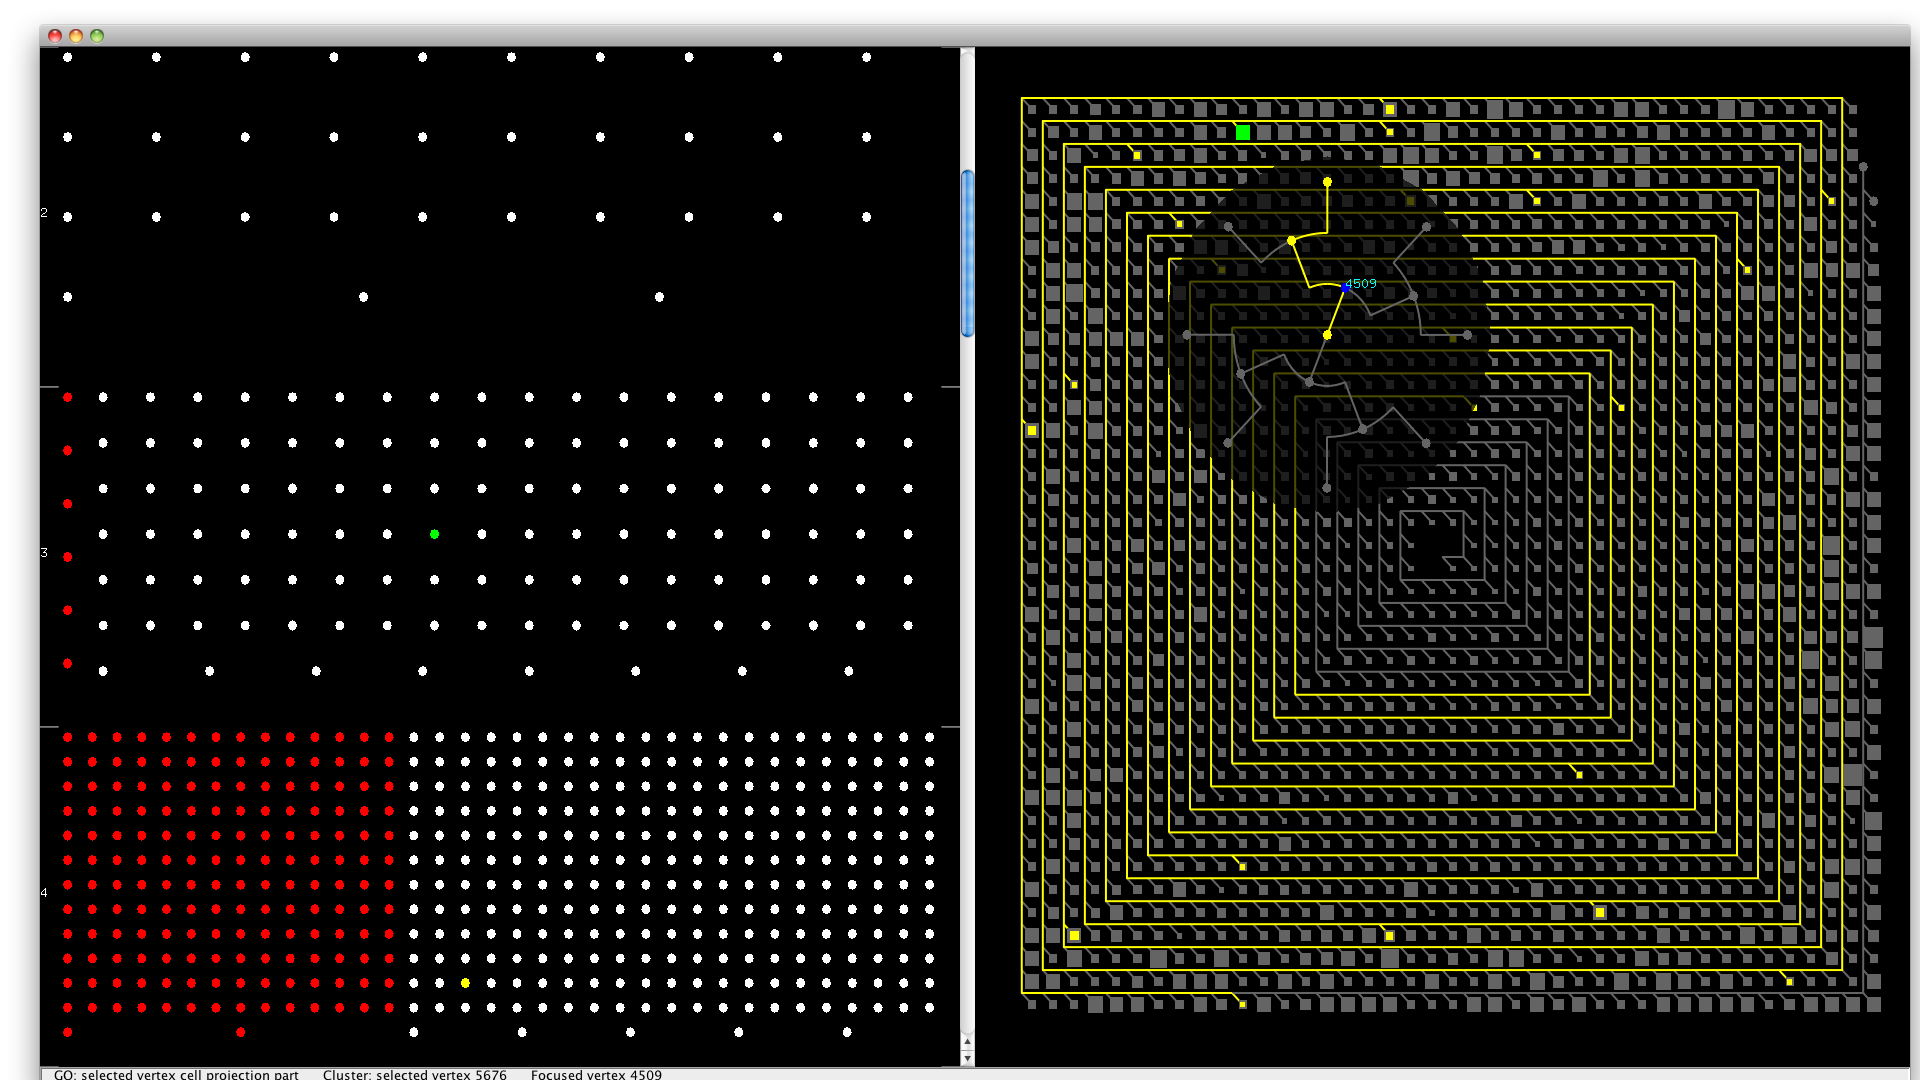
\includegraphics[scale=0.33, angle=90]{pictures/screenshot_3.png}
\caption{Highlighted sub-graph visualization for GO gene ``cell projection part" and Radial lens view of the Cluster grouped vertex ``5676" (green rectangle)}
\end{figure}

\newpage
\begin{figure}[h!]
\centering
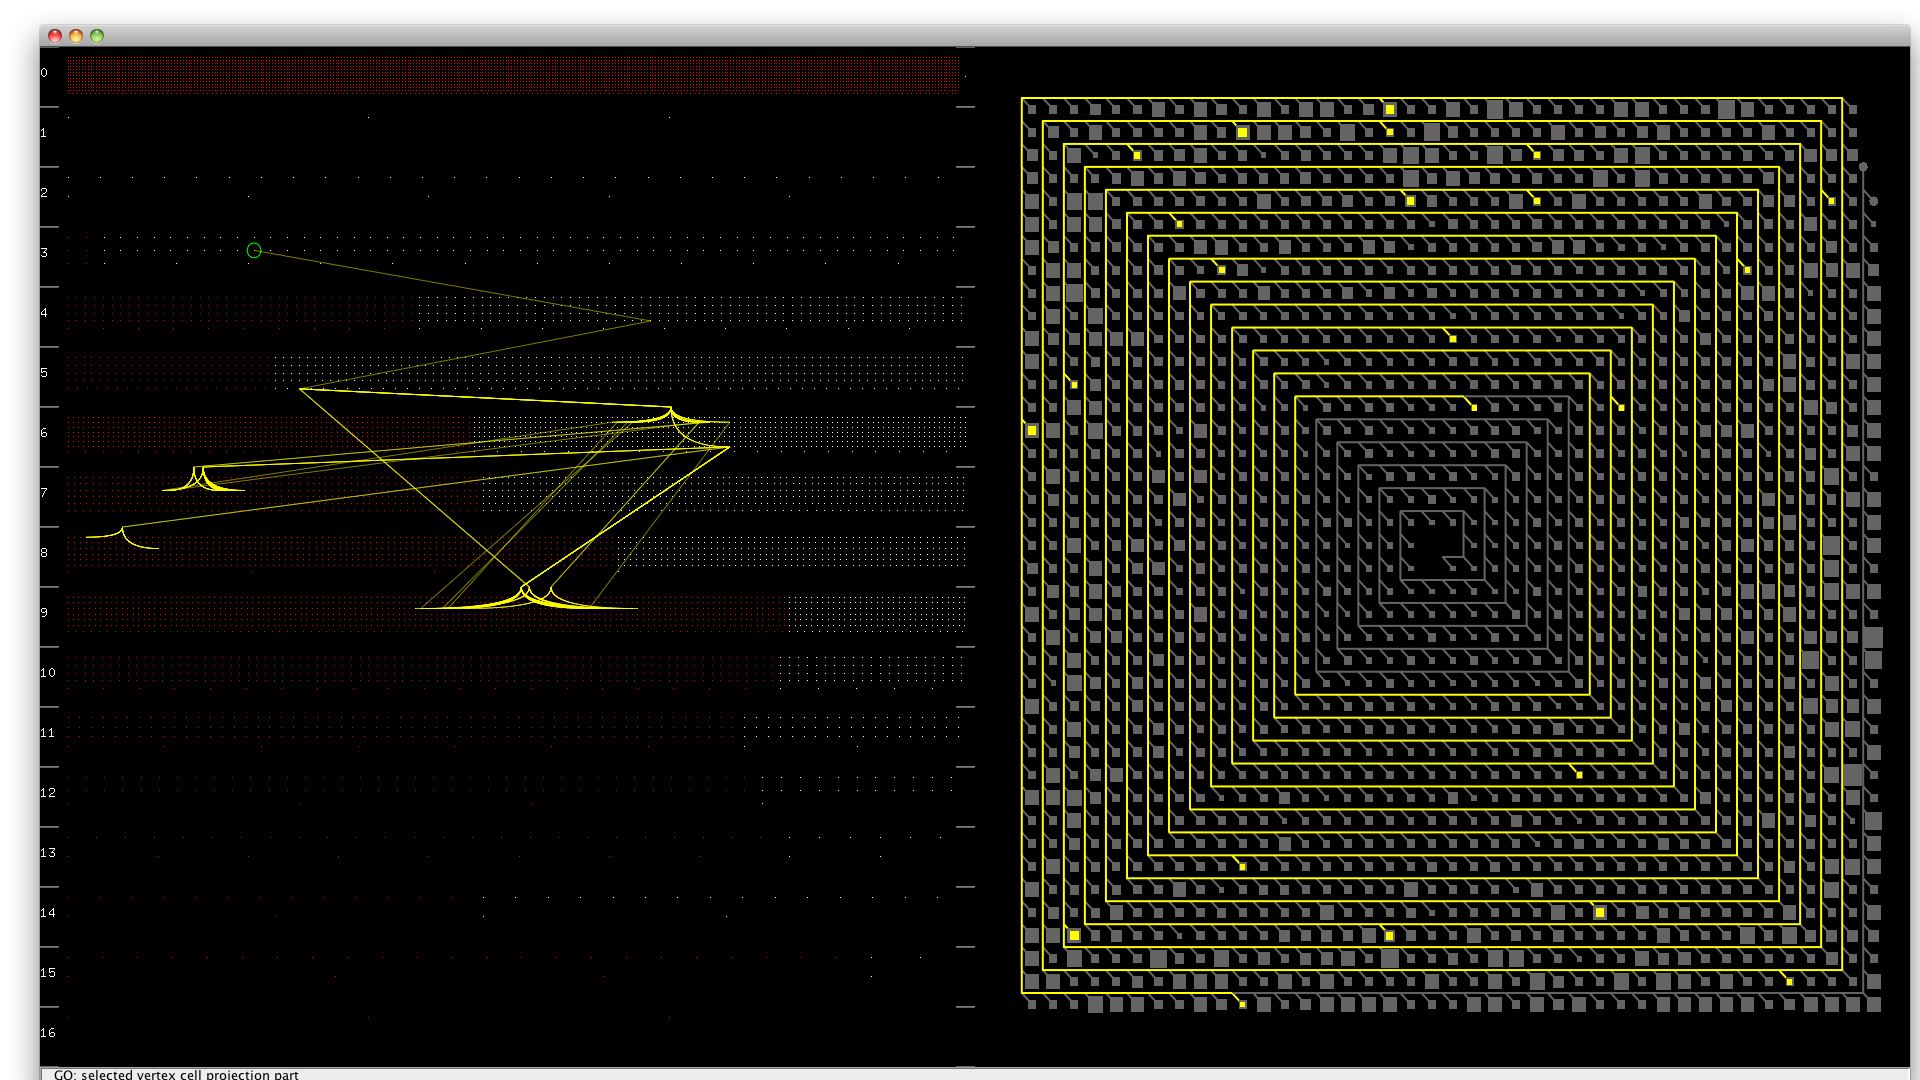
\includegraphics[scale=0.33, angle=90]{pictures/screenshot_4.png}
\caption{Highlighted sub-graph visualization for selected vertex ``cell projection part" (green circle)}
\end{figure}

\newpage
\begin{figure}[h!]
\centering
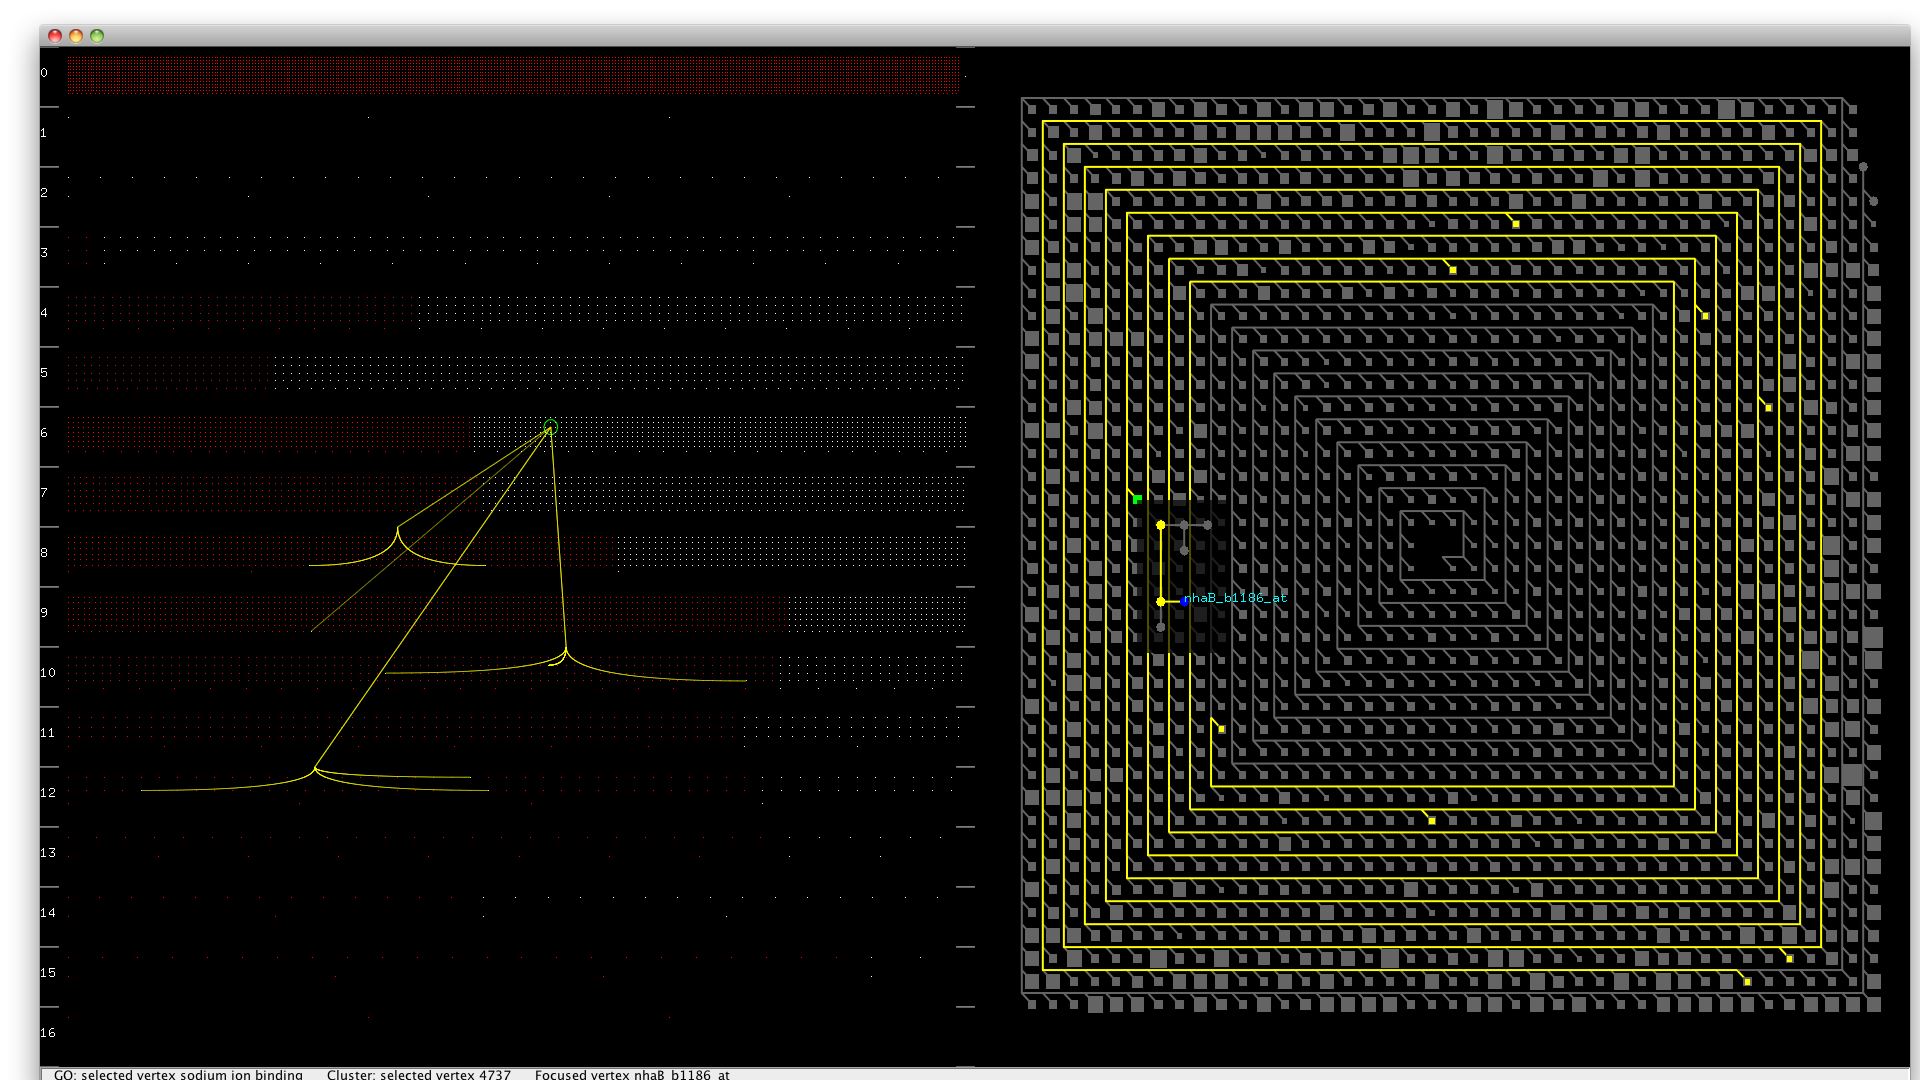
\includegraphics[scale=0.33, angle=90]{pictures/screenshot_5.png}
\caption{Highlighted sub-graph visualization for GO vertex ``sodium ion binding" and Rect lens view of the Cluster grouped vertex ``4737".}
\end{figure}

\newpage
\begin{figure}[h!]
\centering
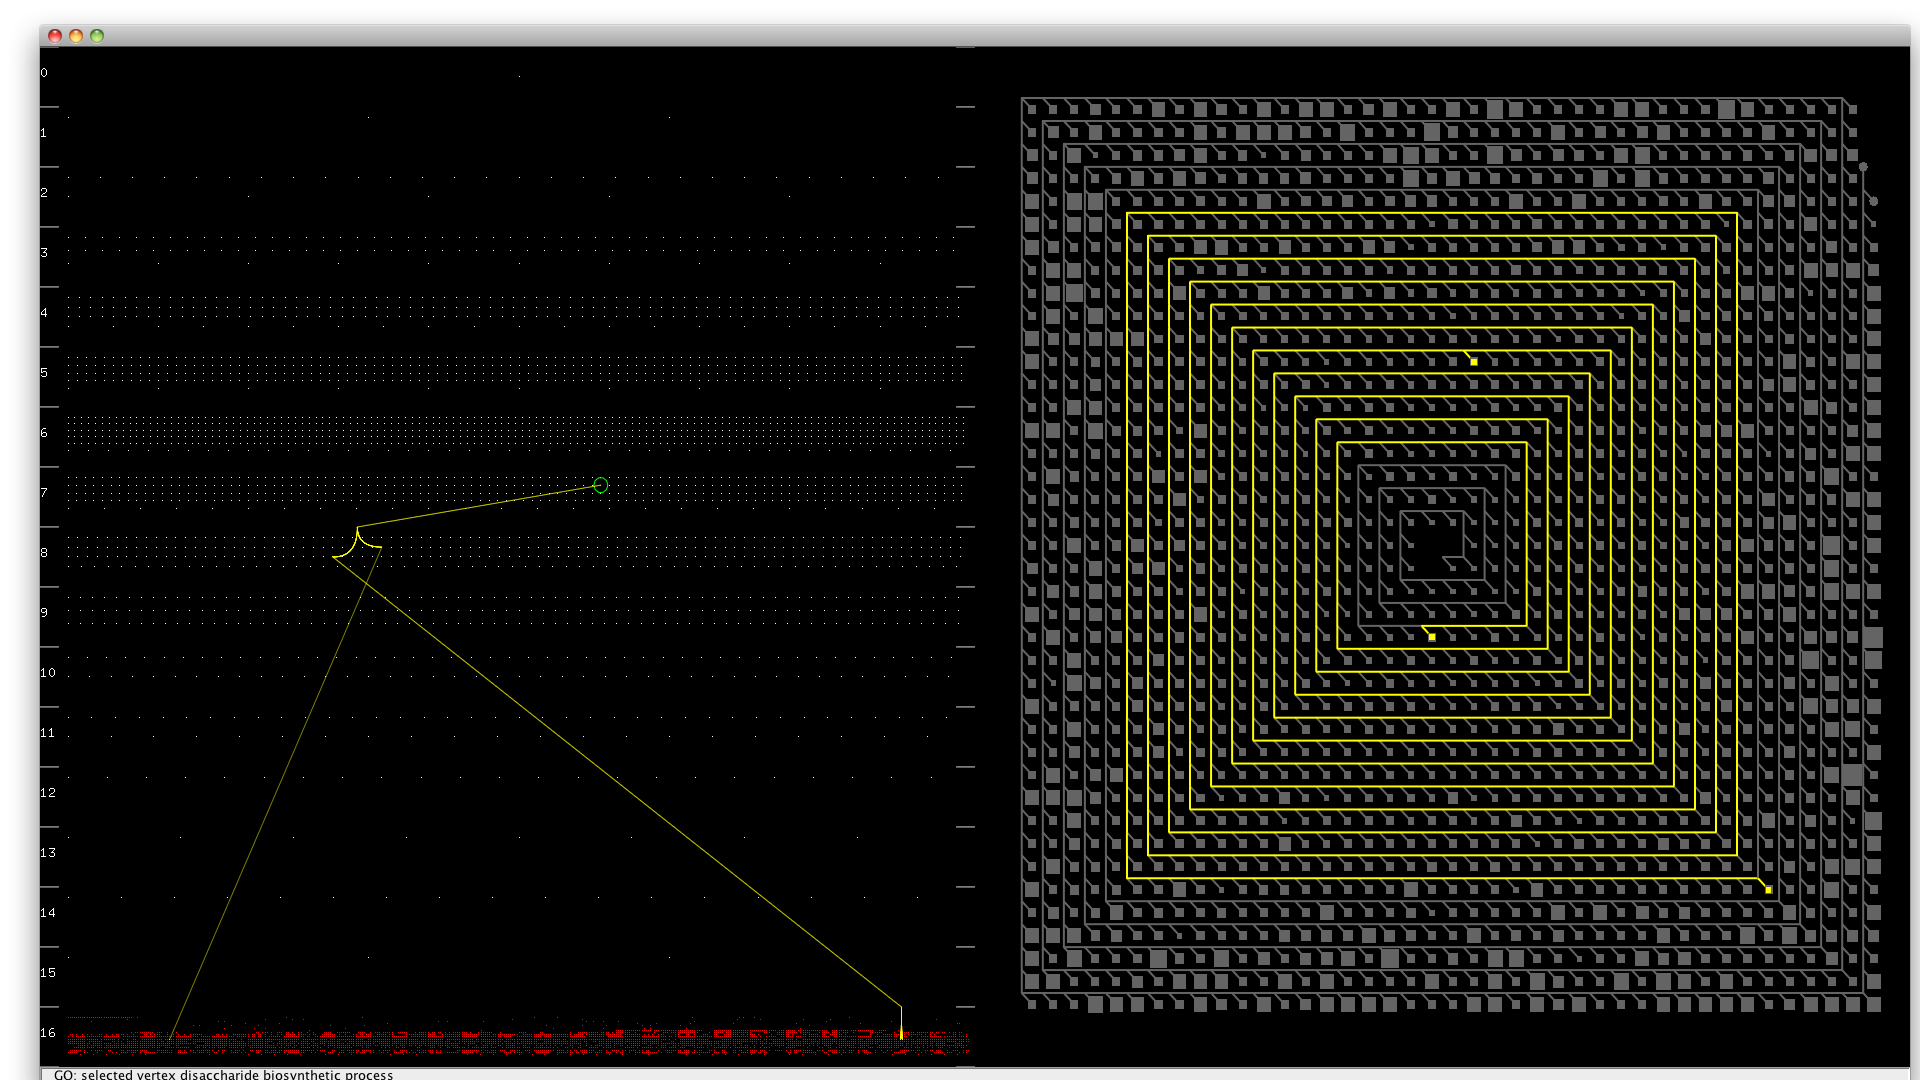
\includegraphics[scale=0.33, angle=90]{pictures/screenshot_6.png}
\caption{Visualization of the Gene Ontology graph using ``Leaf buttom layout" without option ``Show unconnected components" and highlighted sub-graph for the GO vertex ``disaccharide biosynthetic process"}
\end{figure}

\end{document}